% Options for packages loaded elsewhere
\PassOptionsToPackage{unicode}{hyperref}
\PassOptionsToPackage{hyphens}{url}
%
\documentclass[
]{book}
\title{Data Science на R. Лабораторні роботи}
\author{© \href{https://www.linkedin.com/in/valeriy-sydorenko-6782279a/}{Сидоренко В. М.}}
\date{2022-03-08}

\usepackage{amsmath,amssymb}
\usepackage{lmodern}
\usepackage{iftex}
\ifPDFTeX
  \usepackage[T1]{fontenc}
  \usepackage[utf8]{inputenc}
  \usepackage{textcomp} % provide euro and other symbols
\else % if luatex or xetex
  \usepackage{unicode-math}
  \defaultfontfeatures{Scale=MatchLowercase}
  \defaultfontfeatures[\rmfamily]{Ligatures=TeX,Scale=1}
\fi
% Use upquote if available, for straight quotes in verbatim environments
\IfFileExists{upquote.sty}{\usepackage{upquote}}{}
\IfFileExists{microtype.sty}{% use microtype if available
  \usepackage[]{microtype}
  \UseMicrotypeSet[protrusion]{basicmath} % disable protrusion for tt fonts
}{}
\makeatletter
\@ifundefined{KOMAClassName}{% if non-KOMA class
  \IfFileExists{parskip.sty}{%
    \usepackage{parskip}
  }{% else
    \setlength{\parindent}{0pt}
    \setlength{\parskip}{6pt plus 2pt minus 1pt}}
}{% if KOMA class
  \KOMAoptions{parskip=half}}
\makeatother
\usepackage{xcolor}
\IfFileExists{xurl.sty}{\usepackage{xurl}}{} % add URL line breaks if available
\IfFileExists{bookmark.sty}{\usepackage{bookmark}}{\usepackage{hyperref}}
\hypersetup{
  pdftitle={Data Science на R. Лабораторні роботи},
  pdfauthor={© Сидоренко В. М.},
  hidelinks,
  pdfcreator={LaTeX via pandoc}}
\urlstyle{same} % disable monospaced font for URLs
\usepackage{color}
\usepackage{fancyvrb}
\newcommand{\VerbBar}{|}
\newcommand{\VERB}{\Verb[commandchars=\\\{\}]}
\DefineVerbatimEnvironment{Highlighting}{Verbatim}{commandchars=\\\{\}}
% Add ',fontsize=\small' for more characters per line
\usepackage{framed}
\definecolor{shadecolor}{RGB}{248,248,248}
\newenvironment{Shaded}{\begin{snugshade}}{\end{snugshade}}
\newcommand{\AlertTok}[1]{\textcolor[rgb]{0.94,0.16,0.16}{#1}}
\newcommand{\AnnotationTok}[1]{\textcolor[rgb]{0.56,0.35,0.01}{\textbf{\textit{#1}}}}
\newcommand{\AttributeTok}[1]{\textcolor[rgb]{0.77,0.63,0.00}{#1}}
\newcommand{\BaseNTok}[1]{\textcolor[rgb]{0.00,0.00,0.81}{#1}}
\newcommand{\BuiltInTok}[1]{#1}
\newcommand{\CharTok}[1]{\textcolor[rgb]{0.31,0.60,0.02}{#1}}
\newcommand{\CommentTok}[1]{\textcolor[rgb]{0.56,0.35,0.01}{\textit{#1}}}
\newcommand{\CommentVarTok}[1]{\textcolor[rgb]{0.56,0.35,0.01}{\textbf{\textit{#1}}}}
\newcommand{\ConstantTok}[1]{\textcolor[rgb]{0.00,0.00,0.00}{#1}}
\newcommand{\ControlFlowTok}[1]{\textcolor[rgb]{0.13,0.29,0.53}{\textbf{#1}}}
\newcommand{\DataTypeTok}[1]{\textcolor[rgb]{0.13,0.29,0.53}{#1}}
\newcommand{\DecValTok}[1]{\textcolor[rgb]{0.00,0.00,0.81}{#1}}
\newcommand{\DocumentationTok}[1]{\textcolor[rgb]{0.56,0.35,0.01}{\textbf{\textit{#1}}}}
\newcommand{\ErrorTok}[1]{\textcolor[rgb]{0.64,0.00,0.00}{\textbf{#1}}}
\newcommand{\ExtensionTok}[1]{#1}
\newcommand{\FloatTok}[1]{\textcolor[rgb]{0.00,0.00,0.81}{#1}}
\newcommand{\FunctionTok}[1]{\textcolor[rgb]{0.00,0.00,0.00}{#1}}
\newcommand{\ImportTok}[1]{#1}
\newcommand{\InformationTok}[1]{\textcolor[rgb]{0.56,0.35,0.01}{\textbf{\textit{#1}}}}
\newcommand{\KeywordTok}[1]{\textcolor[rgb]{0.13,0.29,0.53}{\textbf{#1}}}
\newcommand{\NormalTok}[1]{#1}
\newcommand{\OperatorTok}[1]{\textcolor[rgb]{0.81,0.36,0.00}{\textbf{#1}}}
\newcommand{\OtherTok}[1]{\textcolor[rgb]{0.56,0.35,0.01}{#1}}
\newcommand{\PreprocessorTok}[1]{\textcolor[rgb]{0.56,0.35,0.01}{\textit{#1}}}
\newcommand{\RegionMarkerTok}[1]{#1}
\newcommand{\SpecialCharTok}[1]{\textcolor[rgb]{0.00,0.00,0.00}{#1}}
\newcommand{\SpecialStringTok}[1]{\textcolor[rgb]{0.31,0.60,0.02}{#1}}
\newcommand{\StringTok}[1]{\textcolor[rgb]{0.31,0.60,0.02}{#1}}
\newcommand{\VariableTok}[1]{\textcolor[rgb]{0.00,0.00,0.00}{#1}}
\newcommand{\VerbatimStringTok}[1]{\textcolor[rgb]{0.31,0.60,0.02}{#1}}
\newcommand{\WarningTok}[1]{\textcolor[rgb]{0.56,0.35,0.01}{\textbf{\textit{#1}}}}
\usepackage{longtable,booktabs,array}
\usepackage{calc} % for calculating minipage widths
% Correct order of tables after \paragraph or \subparagraph
\usepackage{etoolbox}
\makeatletter
\patchcmd\longtable{\par}{\if@noskipsec\mbox{}\fi\par}{}{}
\makeatother
% Allow footnotes in longtable head/foot
\IfFileExists{footnotehyper.sty}{\usepackage{footnotehyper}}{\usepackage{footnote}}
\makesavenoteenv{longtable}
\usepackage{graphicx}
\makeatletter
\def\maxwidth{\ifdim\Gin@nat@width>\linewidth\linewidth\else\Gin@nat@width\fi}
\def\maxheight{\ifdim\Gin@nat@height>\textheight\textheight\else\Gin@nat@height\fi}
\makeatother
% Scale images if necessary, so that they will not overflow the page
% margins by default, and it is still possible to overwrite the defaults
% using explicit options in \includegraphics[width, height, ...]{}
\setkeys{Gin}{width=\maxwidth,height=\maxheight,keepaspectratio}
% Set default figure placement to htbp
\makeatletter
\def\fps@figure{htbp}
\makeatother
\setlength{\emergencystretch}{3em} % prevent overfull lines
\providecommand{\tightlist}{%
  \setlength{\itemsep}{0pt}\setlength{\parskip}{0pt}}
\setcounter{secnumdepth}{5}
\usepackage{booktabs}
\usepackage{amsthm}
\makeatletter
\def\thm@space@setup{%
  \thm@preskip=8pt plus 2pt minus 4pt
  \thm@postskip=\thm@preskip
}
\makeatother
\ifLuaTeX
  \usepackage{selnolig}  % disable illegal ligatures
\fi
\usepackage[]{natbib}
\bibliographystyle{apalike}

\begin{document}
\maketitle

{
\setcounter{tocdepth}{1}
\tableofcontents
}
\hypertarget{ux432ux441ux442ux443ux43f}{%
\chapter{Вступ}\label{ux432ux441ux442ux443ux43f}}

Цей посібник є практичним керіаництвом для виконання лабораторних робіт з дисципліни ``Інтелектуальний аналіз даних'', який викладається в рамках освітньої магістерської програми ``Комп'ютерна інженерія'' спеціальності 123 Комп'ютерна інженерія на кафедрі \href{http://cis.kdu.edu.ua/}{Комп'ютерної інженерії та електроніки} \href{http://www.kdu.edu.ua/}{Кременчуцького національного університету імені Михайла Остроградського}. Автор: Доцент, к. т. н. \href{https://www.linkedin.com/in/valeriy-sydorenko-6782279a/}{Валерій СИДОРЕНКО}.

Мета посібника, який у великій мірі є компілятивним, -- у зручній і адаптованій формі довести новітні технології аналізу даних у середовищі R, спираючись на якісні і відомі першоджерела, зокрема \texttt{vignetts} відповідних програмних пакетів з ресурсу \href{https://cran.r-project.org/}{CRAN}. Тому місцями текст є безпосереднім перекладом з англійської.

Структура посібника спирається на конценпцію міждисциплінарного стандарту CRISP DM \citep{CRISP_DM}, що дає можливість поступово вивчити необхідні інструменти і технології всіх етапів аналізу даних: імпорт та маніпулювання даними, розвідувальний аналіз даних, візуалізація, моделювання та розгортання Data Science-проекту.

Критичні відгуки та зауваження побажання прохання надсилати за адресою \href{mailto:vnsidorenko@gmail.com}{\nolinkurl{vnsidorenko@gmail.com}}.

\hypertarget{modul1}{%
\chapter{Модуль 1. Базовий. Лабораторна робота №1. Створення основи типового Data Science-проєкту}\label{modul1}}

\textbf{Мета:} \emph{``Швидкий старт'' для створення бази Data Science-проекту у середовищі \citep{R-Studio} із застосуванням концепції ``грамотного програмування'' засобами мови програмування \citep{R-base}, пакету RMarkdown та системи комп'ютерної верстки LaTeX}.

\hypertarget{ux449ux43e-ux432ux438-ux431ux443ux434ux435ux442ux435-ux432ux43cux456ux442ux438}{%
\section{Що ви будете вміти?}\label{ux449ux43e-ux432ux438-ux431ux443ux434ux435ux442ux435-ux432ux43cux456ux442ux438}}

\begin{itemize}
\tightlist
\item
  виконувати експорт/імпорт даних, елеменарну їх обробку, візуалізацію даних та результатів обчислень засобами мови R у середовищі IDE RStudio.
\item
  Створювати електронний документ (у форматах html, pdf, doc) на кшталт того, \textbf{який ви зараз читаєте} (інтерактивне меню, можливість показати/сховати код і т. ін.).
\item
  використовувати засоби редактору LaTeX для набору формул, наприклад, як ця: \(y(x)=b_0+b_1x+b_2x^2\).
\item
  створювати бібліографічну базу даних засобами \href{https://ru.wikipedia.org/wiki/BibTeX}{BibTeX}, яка автоматично формує розділ посилань `References', як \textbf{у цьому документі}.
\end{itemize}

\hypertarget{ux43aux43eux440ux43eux442ux43aux456-ux442ux435ux43eux440ux435ux442ux438ux447ux43dux456-ux432ux456ux434ux43eux43cux43eux441ux442ux456}{%
\section{Короткі теоретичні відомості}\label{ux43aux43eux440ux43eux442ux43aux456-ux442ux435ux43eux440ux435ux442ux438ux447ux43dux456-ux432ux456ux434ux43eux43cux43eux441ux442ux456}}

\hypertarget{ux449ux43e-ux442ux430ux43aux435-data-science-ux43fux440ux43eux435ux43aux442}{%
\subsection{Що таке Data Science-проект?}\label{ux449ux43e-ux442ux430ux43aux435-data-science-ux43fux440ux43eux435ux43aux442}}

Будь-який Data Science-проект (альтернативна назва -- Data Mining-проект) має на меті реалізацію на практиці методології \href{https://www.the-modeling-agency.com/crisp-dm.pdf}{CRISP DM} \citep{CRISP_DM}. Згідно зі стандартом CRISP-DM 1.0 життєвий цикл проекту Data Mining має складатися з шести фаз (рис. 1):\\
- розуміння бізнес-процесів (business understanding);\\
- розуміння даних (data understanding);\\
- підготовка даних (data preparation);\\
- моделювання (modeling);\\
- оцінка (evaluation);\\
- розміщення (deployment).

\begin{figure}
\centering
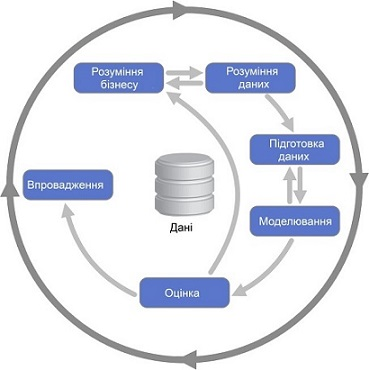
\includegraphics{image/CRISP_DM.jpg}
\caption{\emph{Рис. 1. Життєвий цикл процесу Data Mining згідно з методологією CRISP }}
\end{figure}

\textbf{Фаза розуміння} бізнес-процесів включає наступні задачі:\\
- визначення бізнес-цілей;\\
- визначення ситуації;\\
- визначення цілей Data Mining;\\
- створення плану проекта.\\
\textbf{Фаза розуміння} даних включає наступні задачі:\\
- первинний збір даних;\\
- опис даних;\\
- вивчення даних;\\
- перевірка якості даних.\\
\textbf{Фаза підготовки} даних включає в себе всі дії, пов'язані з остаточним формуванням набору даних для аналізу. При цьому виконуються п'ять задач:\\
- вибір даних;\\
- очищення даних;\\
- конструювання даних;\\
- інтеграція даних;\\
- форматування даних.\\
\textbf{Фаза моделювання} -\/-- призначена для вибору оптимального методу побудови моделей і настроювання його параметрів для отримання оптимальних рішень. На даній фазі вирішуються наступні задачі:\\
- вибір методу моделювання;\\
- генерація тестового проекту;\\
- створення моделей;\\
- оцінка моделей.\\
\textbf{Фаза оцінки} -\/-- призвана більш ґрунтовно оцінити модель до процесу її остаточного розміщення, щоб впевнитись у досяжності поставлених бізнес-цілей. Дана фаза включає наступні задачі:\\
- оцінка результатів;\\
- перегляд процесу;\\
- визначення подальших дій.\\
\textbf{Фаза розміщення} передбачає розгортання моделі.

Якщо виділити з даного процесу суто технологічну складову, то типова технологічна основа будь-якого Data Science-проекту має виглядати наступним чином \citep{r4ds} (рис. 2).

\begin{figure}
\centering
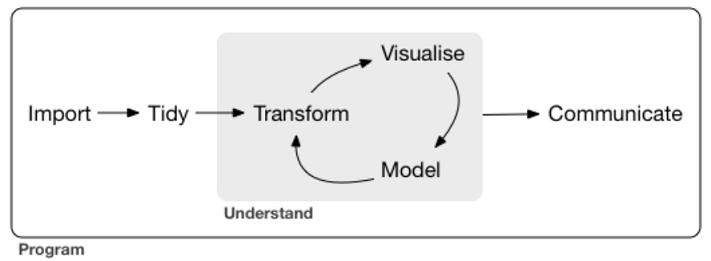
\includegraphics{image/process_DS.png}
\caption{\emph{Рис. 2. Структура типового Data Science-проекту}}
\end{figure}

Перша задача \emph{імпорту даних} (\textbf{Import}) полягає у вилученні необхідних сирих даних з будь-яких джерел (файли, БД, дані з датчиків у реальному часі і т. ін) самого різного формату.

Друга задача (\textbf{Tidy}) -- \emph{приведення даних до} так званого \emph{``охайного'' вигляду}, придатного для аналізу. Як правило мова йде про приведення даних до табличного вигляду ``ключ-значення'', або, іншими словами, ``об'єкт-ознака''. Дана процедура є частиною більш загальної задачі підготовки даних до аналізу (\textbf{Wrangling, Munging}), яка включає інші процедури, наприклад, заповнення пропущених значень (Missing Value Emputation), вилучення неінформативних даних (data reduction), різного роду трансформації (\textbf{Transforming}) і т. ін. Тобто, \textbf{Tiding+Transforming=Wrangling(Munging)}.

Тріада задач \emph{трансформація-візуалізація-моделювання} (\textbf{Transform-Visualise-Model}) складають ядро Data Mining-процесу, суть якого полягає в пошуку нетривіальних практично корисних закономірностей в даних, шляхом висування і перевірки гіпотез, побудови різного роду моделей, який обов'язково супроводжується візуалізацією як проміжних, так і кінцевих результатів моделювання, що предоставляються замовнику. Саме ця тріада задач забезпечує фази розуміння (\textbf{Understanding}) даних, моделей та паттернів, що знаходяться в даних і створюють основу монетизованого продукту інтелектуального аналізу даних.

Останній етап -- представлення проміжних чи остаточних результатів інтелектуального аналізу даних (\textbf{Сommunicate}) іншим членам команди, які задіяні у проекті, у зручному для сприйняття вигляді з використанням прози, таблиць, графіків та коду.

Для реалізації типового Data Science-проекту необхідний відповідний інструментарій, який би був гнучким і задовольняв всім необхідним вимогам, котрих потребують вищезгадані задачі, і давав би можливість розв'язати будь-яку задачу без значних витрат часу, в першу чергу, на маніпулювання даними та підготовку результатів.

Мова і середовище програмування R з великим арсеналом програмних пакетів, IDE RStudio та технологія так званого \emph{грамотного програмування} дозволяє ефективну реалізацію всіх етапів типового Data Science-проекту, об'єднавши всі задачі в єдине ціле.

\hypertarget{ux43aux43eux43dux446ux435ux43fux446ux456ux44f-ux433ux440ux430ux43cux43eux442ux43dux43eux433ux43e-ux43fux440ux43eux433ux440ux430ux43cux443ux432ux430ux43dux43dux44f}{%
\subsection{Концепція грамотного програмування}\label{ux43aux43eux43dux446ux435ux43fux446ux456ux44f-ux433ux440ux430ux43cux43eux442ux43dux43eux433ux43e-ux43fux440ux43eux433ux440ux430ux43cux443ux432ux430ux43dux43dux44f}}

Представлення проміжних чи остаточних результатів проекту може бути виконано у тому чи іншому вигляді -- звіту, презентації, методичних вказівок, наукової статті тощо, в одному з поширених форматів -- .doc, pdf, .html тощо.

Протягом багатьох років у наукових та ділових колах стандартом де-факто є застосування так званої парадигми \href{https://en.wikipedia.org/wiki/Literate_programming}{\emph{грамотного програмування}} для підготовки електронних документів з використанням у тому числі і потужніх засобів комп'ютерної графіки. З виникненням і розвитком Data Science, методологію грамотного програмування було взято на озброєння і реалізоване практично в кожному потужному інструменті Data Science.

\emph{Грамотне програмування} (Literate Programming) -- концепція, методологія програмування і документування, в якій програма складається з прози на природній мові упереміж з макропідстановками і кодом на мовах програмування.

В основі технології грамотного програмування лежить поняття \emph{динамічного документу} -- текстового документу, який складається з тексту та коду, з використанням необхідних мов програмування, який дозволяє згенерувати власне електронний документ заданого формату. При цьому використовуються як можливості мов розмітки документів (напр. Markdown, YAML, HTML, LaTeX), так і можливості доступу до потужних програмних бібліотек, призначених для обробки даних та комп'ютерної графіки.

Таким чином, логічно мати певне програмне середовище, яке дозволить поєднати низку таких технологій разом і створити зручний інтерфейс розробника. Існують різні програмні засоби і середовища \href{https://uk.wikipedia.org/wiki/\%D0\%86\%D0\%BD\%D1\%82\%D0\%B5\%D0\%B3\%D1\%80\%D0\%BE\%D0\%B2\%D0\%B0\%D0\%BD\%D0\%B5_\%D1\%81\%D0\%B5\%D1\%80\%D0\%B5\%D0\%B4\%D0\%BE\%D0\%B2\%D0\%B8\%D1\%89\%D0\%B5_\%D1\%80\%D0\%BE\%D0\%B7\%D1\%80\%D0\%BE\%D0\%B1\%D0\%BA\%D0\%B8}{(IDE, Integrated Development Environment, інтегроване середовище розробки)}, що дозволяють реалізувати технологію грамотного програмування.

У даній лабораторній роботі пропонується низка наразі актуальних і популярних інструментів для створення динамічних документів (рис. 3):

\begin{itemize}
\item
  IDE \href{https://www.rstudio.com/}{R Studio} \citep{R-Studio} як інтегроване середовище розробки;
\item
  спеціалізовану мову програмування \href{https://cran.r-project.org/}{R} \citep{R-base} та арсенал її потужніх бібліотек -- для маніпулювання даними та візуалізації результатів;
\item
  фреймворк \href{http://rmarkdown.rstudio.com/}{RMarkdown} \citep{R-rmarkdown} -- для підготовки динамічних звітів мовою розмітки \href{https://uk.wikipedia.org/wiki/Markdown}{Markdown}; (див.\citep{CheatSheetMarkdown} та шпаргалку у RStudio: \emph{``Help\textbackslash Cheat\_Sheets''}); також покрокове керівництво \href{https://rpubs.com/domelia/828777}{Д. Омельченко}; також див. \href{https://rpubs.com/domelia/834925}{R Markdown: продолжение. Подготовка рукописи научной статьи};
\item
  мову розмітки даних \href{https://uk.wikipedia.org/wiki/LaTeX}{LaTex} для високоякісного оформлення наукових документів.
\end{itemize}

\begin{figure}
\centering
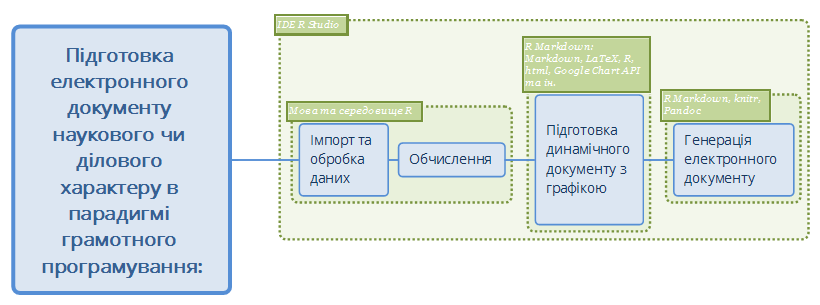
\includegraphics{image/process.png}
\caption{\emph{Рис. 3. Структура процесу підготовки електронного документу наукового чи ділового характеру в парадигмі грамотного програмування (literate programming)}}
\end{figure}

\hypertarget{markdown-ux456-rmarkdown}{%
\subsection{Markdown і RMarkdown}\label{markdown-ux456-rmarkdown}}

\textbf{Markdown} (МФА: {[}маркдаун{]}) -- полегшена мова розмітки даних, яку створено з ухилом на прочитність та зручність у публікації з подальшим перетворенням її на structurally valid XHTML або HTML.

Такі сайти, як GitHub, Reddit та Stack Overflow використовують Markdown для полегшення обговорень між користувачами.

\textbf{R Markdown} \citep{RMark} -- фреймворк R, який дозволяє створювати динамічні Markdown-документи у середовищі IDE RStudio в стилі грамотного програмування з використанням всіх можливих потужностей мови R та її бібліотек. Дозволяє реалізовувати інтерфейс так званих ноутбуків для створення документів з текстом та кодом разом для виготовлення елегантно відформатованого виводу. Дозволяє використовувати декілька мов, включаючи R, Python, С++, HTML, SQL, \href{http://mc-stan.org/}{Stan}. Через конвертор \href{http://pandoc.org/}{Pandoc} дозволяє здійснювати вивід у html, doc або pdf формат у вигляді веб-сторінок, брошюр, буклетів, слайдів.

\hypertarget{ux456ux43dux441ux442ux430ux43bux44fux446ux456ux44f-r}{%
\subsection{Інсталяція R}\label{ux456ux43dux441ux442ux430ux43bux44fux446ux456ux44f-r}}

Для цього необхідно зайти на \href{https://cran.r-project.org/}{CRAN}, скачати і встановити актуальну версію R. Даний дистрибутив R має свій GUI, однак його можливості досить обмежені. Тут, у розділі `Contributed', також можна знайти безліч цікавої літератури, написаної різними мовами.

Одне з найкоротших і доступних введень у мову R можна знайти на сторінці \href{http://dkhramov.dp.ua/Comp.R.html\#.Wpetc1rFJdj}{Дмитра Храмова}. Зокрема, знайомство з \href{http://dkhramov.dp.ua/images/edu/Stu.WebMining/ch04_graphics.pdf}{елементами базової графіки}.

\hypertarget{ux456ux43dux441ux442ux430ux43bux44fux446ux456ux44f-rstudio}{%
\subsection{Інсталяція RStudio}\label{ux456ux43dux441ux442ux430ux43bux44fux446ux456ux44f-rstudio}}

Для зручної роботи і відладки програм, зокрема роботи з фреймворком RMarkdown для створення динамічного документу, необхідно встановити IDE \href{https://www.rstudio.com/products/rstudio/download/}{RStudio}.

\hypertarget{CreateRMarkdown}{%
\subsection{Створення RMarkdown-документу}\label{CreateRMarkdown}}

\begin{enumerate}
\def\labelenumi{\arabic{enumi}.}
\item
  Завантажити RStudio.
\item
  Створити RMarkdown-документ у форматі \href{http://rmarkdown.rstudio.com/r_notebooks.html}{R Notebook}, вибравши відповідний пункт \href{https://prnt.sc/gkpes4}{меню}.
\end{enumerate}

\hypertarget{ux433ux435ux43dux435ux440ux430ux446ux456ux44f-ux435ux43bux435ux43aux442ux440ux43eux43dux43dux43eux433ux43e-ux434ux43eux43aux443ux43cux435ux43dux442ux443}{%
\subsection{Генерація електронного документу}\label{ux433ux435ux43dux435ux440ux430ux446ux456ux44f-ux435ux43bux435ux43aux442ux440ux43eux43dux43dux43eux433ux43e-ux434ux43eux43aux443ux43cux435ux43dux442ux443}}

Генерація електронного документу здійснюється натисканням комбінації \emph{Ctrl+Shift+K}.

\hypertarget{ux43fux440ux438ux43aux43bux430ux434-ux441ux442ux432ux43eux440ux435ux43dux43dux44f-markdown-ux434ux43eux43aux443ux43cux435ux43dux442ux443}{%
\section{Приклад створення Markdown-документу}\label{ux43fux440ux438ux43aux43bux430ux434-ux441ux442ux432ux43eux440ux435ux43dux43dux44f-markdown-ux434ux43eux43aux443ux43cux435ux43dux442ux443}}

\hypertarget{ux43fux43eux441ux442ux430ux43dux43eux432ux43aux430-ux437ux430ux434ux430ux447ux456}{%
\subsection{Постановка задачі}\label{ux43fux43eux441ux442ux430ux43dux43eux432ux43aux430-ux437ux430ux434ux430ux447ux456}}

Побудувати графік функції \(y(x)=b_ox+b_1+b_2x^2\) для діапазону \(x \in [x_1;x_2]\).

\hypertarget{ux432ux438ux43aux43eux43dux430ux43dux43dux44f-ux437ux430ux432ux434ux430ux43dux43dux44f}{%
\subsection{Виконання завдання}\label{ux432ux438ux43aux43eux43dux430ux43dux43dux44f-ux437ux430ux432ux434ux430ux43dux43dux44f}}

\begin{enumerate}
\def\labelenumi{\arabic{enumi}.}
\item
  Створюємо документ R Markdown, як описано вище у п. \protect\hyperlink{CreateRMarkdown}{\emph{Створення RMarkdown-документу}}.
\item
  Налаштовуємо потрібним чином YAML-заголовок документу, у якому задаються метадані всього документу (рис. 4).
\end{enumerate}

\begin{figure}
\centering
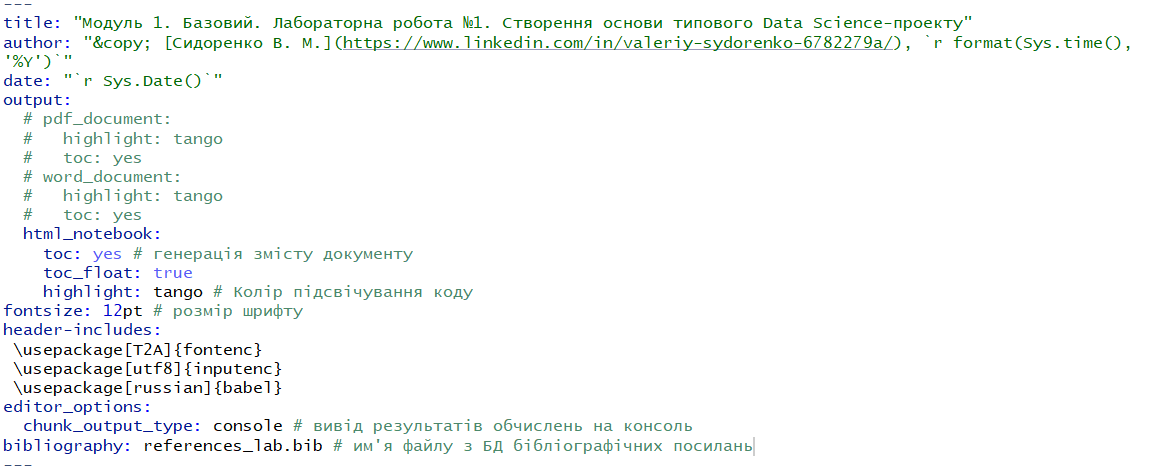
\includegraphics{image/YAML.png}
\caption{\emph{Рис. 4. Вигляд YAML-заголовку для документу, який ви зараз читаєте}}
\end{figure}

\begin{enumerate}
\def\labelenumi{\arabic{enumi}.}
\setcounter{enumi}{2}
\tightlist
\item
  Для набору формул використовуємо \texttt{LaTeX} згідно з правилами \href{https://en.wikibooks.org/wiki/LaTeX/Mathematics}{його синтаксису}. Формула у RMarkdown-документі має бути взята у символи \$:
\end{enumerate}

\texttt{\$y(x)=b\_ox+b\_1+b\_2x\^{}2\$}

\begin{enumerate}
\def\labelenumi{\arabic{enumi}.}
\setcounter{enumi}{2}
\tightlist
\item
  Пишемо код на R засобами базової графіки у відповідній зоні, яка називається чанком @ref(fig:fig\_1):
\end{enumerate}

\begin{Shaded}
\begin{Highlighting}[]
\CommentTok{\# Задаємо параметри функції}
\NormalTok{b0 }\OtherTok{\textless{}{-}} \DecValTok{2}
\NormalTok{b1 }\OtherTok{\textless{}{-}} \DecValTok{3}
\NormalTok{b2 }\OtherTok{\textless{}{-}} \FloatTok{1.57}

\CommentTok{\# Задаємо область визначення}

\NormalTok{x }\OtherTok{\textless{}{-}} \FunctionTok{seq}\NormalTok{(}\SpecialCharTok{{-}}\DecValTok{1}\NormalTok{, }\DecValTok{1}\NormalTok{, .}\DecValTok{1}\NormalTok{)}
\NormalTok{y }\OtherTok{\textless{}{-}}\NormalTok{ b0 }\SpecialCharTok{+}\NormalTok{ b1 }\SpecialCharTok{*}\NormalTok{ x }\SpecialCharTok{+}\NormalTok{ b2 }\SpecialCharTok{*}\NormalTok{ x}\SpecialCharTok{\^{}}\DecValTok{2}

\FunctionTok{plot}\NormalTok{(x, y,}
     \AttributeTok{type =} \StringTok{"l"}\NormalTok{,}
     \AttributeTok{col =} \StringTok{"red"}\NormalTok{,}
     \AttributeTok{main =} \StringTok{"Графік функції"}\NormalTok{,}
     \AttributeTok{xlab =} \StringTok{"x"}\NormalTok{,}
     \AttributeTok{ylab =} \StringTok{"y"}
\NormalTok{     )}
\end{Highlighting}
\end{Shaded}

\begin{verbatim}
## Warning in title(...): font width unknown for character 0xc3
\end{verbatim}

\begin{verbatim}
## Warning in title(...): font width unknown for character 0xf0
\end{verbatim}

\begin{verbatim}
## Warning in title(...): font width unknown for character 0xe0
\end{verbatim}

\begin{verbatim}
## Warning in title(...): font width unknown for character 0xf4
\end{verbatim}

\begin{verbatim}
## Warning in title(...): font width unknown for character 0xb3
\end{verbatim}

\begin{verbatim}
## Warning in title(...): font width unknown for character 0xea
\end{verbatim}

\begin{verbatim}
## Warning in title(...): font width unknown for character 0xf4

## Warning in title(...): font width unknown for character 0xf4
\end{verbatim}

\begin{Shaded}
\begin{Highlighting}[]
\FunctionTok{points}\NormalTok{(x, y,}
       \AttributeTok{col =} \StringTok{"blue"}\NormalTok{)}
\end{Highlighting}
\end{Shaded}

\begin{figure}

{\centering 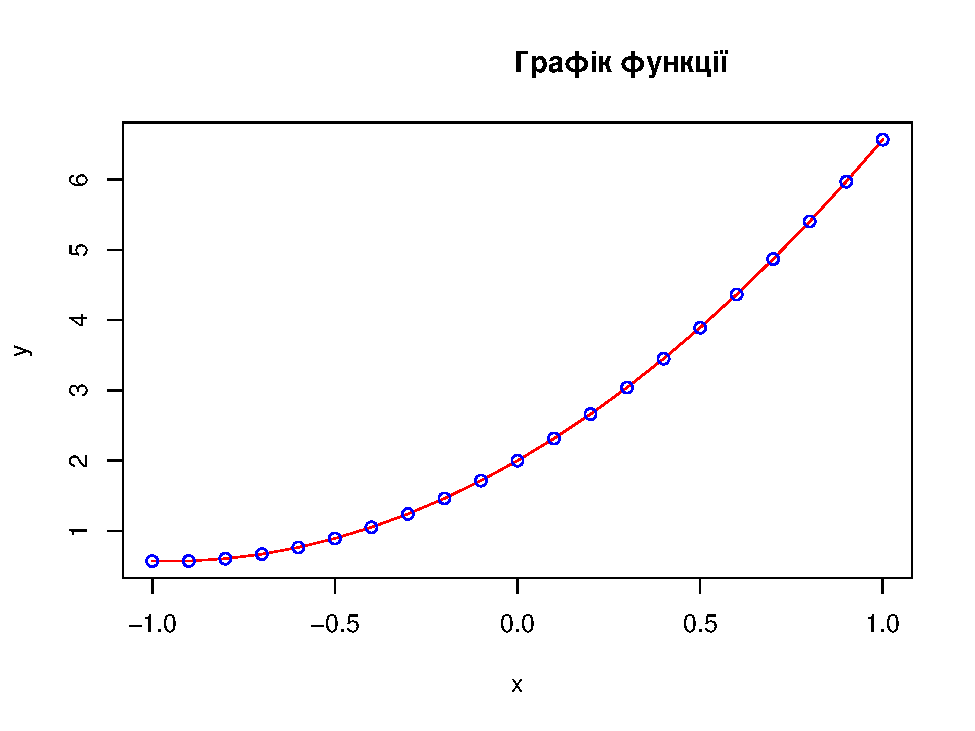
\includegraphics[width=0.8\linewidth]{DS-book-lab_files/figure-latex/fig_1-1} 

}

\caption{Example fig.}(\#fig:fig_1)
\end{figure}

\begin{Shaded}
\begin{Highlighting}[]
\NormalTok{df }\OtherTok{\textless{}{-}} \FunctionTok{data.frame}\NormalTok{(}\AttributeTok{x =}\NormalTok{ x, }\AttributeTok{y =}\NormalTok{ y) }\CommentTok{\# створюємо таблицю даних}
\end{Highlighting}
\end{Shaded}

\begin{enumerate}
\def\labelenumi{\arabic{enumi}.}
\setcounter{enumi}{3}
\tightlist
\item
  Продемонструємо можливості пакету \texttt{rio} \citep{R-rio} для експорту (імпорту) даних на диск (з диску).
\end{enumerate}

\begin{Shaded}
\begin{Highlighting}[]
\CommentTok{\# install.packages("rio") \# інсталяція пакету}
\FunctionTok{library}\NormalTok{(rio) }\CommentTok{\# підключення пакету}
\FunctionTok{export}\NormalTok{(df, }\StringTok{"data/data.csv"}\NormalTok{)}
\end{Highlighting}
\end{Shaded}

\begin{enumerate}
\def\labelenumi{\arabic{enumi}.}
\setcounter{enumi}{4}
\tightlist
\item
  Виконуємо імпорт даних із файлу і візуалізацію у вигляді таблиці @ref(tab:tab\_1).
\end{enumerate}

\begin{Shaded}
\begin{Highlighting}[]
\NormalTok{dfNew }\OtherTok{\textless{}{-}}  \FunctionTok{import}\NormalTok{(}\StringTok{"data/data.csv"}\NormalTok{)}

\CommentTok{\# Таблиця засобами knitr}
\NormalTok{knitr}\SpecialCharTok{::}\FunctionTok{kable}\NormalTok{(}\FunctionTok{head}\NormalTok{(dfNew),}
             \AttributeTok{caption =} \StringTok{"\_Табл. 1. Фрагмент таблиці даних\_"}\NormalTok{)}
\end{Highlighting}
\end{Shaded}

\begin{table}

\caption{(\#tab:tab_1)_Табл. 1. Фрагмент таблиці даних_}
\centering
\begin{tabular}[t]{r|r}
\hline
x & y\\
\hline
-1.0 & 0.5700\\
\hline
-0.9 & 0.5717\\
\hline
-0.8 & 0.6048\\
\hline
-0.7 & 0.6693\\
\hline
-0.6 & 0.7652\\
\hline
-0.5 & 0.8925\\
\hline
\end{tabular}
\end{table}

\begin{Shaded}
\begin{Highlighting}[]
\CommentTok{\# Таблиця засобами stargazer}
\CommentTok{\# stargazer::stargazer(head(dfNew),}
\CommentTok{\#                      type = "html",}
\CommentTok{\#                      summary = FALSE,}
\CommentTok{\#              title = "\_Табл. 1. Фрагмент таблиці даних\_")}


\CommentTok{\# Таблиця засобами xtable}
\CommentTok{\# print(xtable::xtable(head(dfNew),}
\CommentTok{\#                      type = "html",}
\CommentTok{\#                      html.table.attributes="border=0",}
\CommentTok{\#                      summary = FALSE,}
\CommentTok{\#              caption = "\_Табл. 1. Фрагмент таблиці даних\_"))}
\end{Highlighting}
\end{Shaded}

\begin{enumerate}
\def\labelenumi{\arabic{enumi}.}
\setcounter{enumi}{5}
\tightlist
\item
  Формуємо результуючу таблицю.
\end{enumerate}

\emph{Табл. 2. Параметри функції}

\begin{longtable}[]{@{}ll@{}}
\toprule
Параметр & Значення \\
\midrule
\endhead
\(b_0\) & 2 \\
\(b_1\) & 3 \\
\(b_2\) & 1.57 \\
\(x_1\) & -1 \\
\(x_2\) & 1 \\
\bottomrule
\end{longtable}

\hypertarget{ux456ux43dux434ux438ux432ux456ux434ux443ux430ux43bux44cux43dux456-ux437ux430ux432ux434ux430ux43dux43dux44f-ux43dux430-ux43bux430ux431ux43eux440ux430ux442ux43eux440ux43dux443-ux440ux43eux431ux43eux442ux443}{%
\subsection{Індивідуальні завдання на лабораторну роботу}\label{ux456ux43dux434ux438ux432ux456ux434ux443ux430ux43bux44cux43dux456-ux437ux430ux432ux434ux430ux43dux43dux44f-ux43dux430-ux43bux430ux431ux43eux440ux430ux442ux43eux440ux43dux443-ux440ux43eux431ux43eux442ux443}}

Видає викладач.

\hypertarget{ux434ux43eux43cux430ux448ux43dux454-ux437ux430ux432ux434ux430ux43dux43dux44f}{%
\subsection{Домашнє завдання}\label{ux434ux43eux43cux430ux448ux43dux454-ux437ux430ux432ux434ux430ux43dux43dux44f}}

\begin{enumerate}
\def\labelenumi{\arabic{enumi}.}
\item
  Ознайомитися з можливостями пакету \texttt{ggplot2} \citep{ggplot2}.
\item
  Оптимізувати код, наведений у даній методичці, за допомогою потокового оператора \texttt{\%\textgreater{}\%} засобами пакету \texttt{ggplot2}.
\item
  Побудувати графік функції засобами пакету \texttt{ggplot2}. \citep{A3}
\end{enumerate}

\hypertarget{ux43bux430ux431ux43eux440ux430ux442ux43eux440ux43dux430-ux440ux43eux431ux43eux442ux430-2.-ux43cux430ux43dux456ux43fux443ux43bux44eux432ux430ux43dux43dux44f-ux434ux430ux43dux438ux43cux438}{%
\chapter{Лабораторна робота №2. Маніпулювання даними}\label{ux43bux430ux431ux43eux440ux430ux442ux43eux440ux43dux430-ux440ux43eux431ux43eux442ux430-2.-ux43cux430ux43dux456ux43fux443ux43bux44eux432ux430ux43dux43dux44f-ux434ux430ux43dux438ux43cux438}}

\textbf{Мета:} \emph{Засвоєння принципів, знайомвство з інструментами та набуття навичок манпулювання даними (\textbf{wrangle}) засобами мови програмування \texttt{R} та колекції пакетів \citep{R-tidyverse}.}

\hypertarget{ux449ux43e-ux432ux438-ux431ux443ux434ux435ux442ux435-ux432ux43cux456ux442ux438-1}{%
\section{Що ви будете вміти?}\label{ux449ux43e-ux432ux438-ux431ux443ux434ux435ux442ux435-ux432ux43cux456ux442ux438-1}}

\begin{itemize}
\tightlist
\item
  виконувати імпорт даних з файлів різного формату, включаючи реляційні бази даних засобами мови R у середовищі IDE RStudio.
\item
  обробляти пропущені значення та приводити дані до ``охайного'' вигляду за допомогою пакету \citep{R-tidyr}.
\item
  маніпулювати даними засобами мови R у середовищі IDE RStudio в парадигмі пакету \citep{R-dplyr} з використанням потокового оператору \texttt{\%\textgreater{}\%}.
\end{itemize}

\hypertarget{ux43aux43eux440ux43eux442ux43aux456-ux442ux435ux43eux440ux435ux442ux438ux447ux43dux456-ux432ux456ux434ux43eux43cux43eux441ux442ux456-1}{%
\section{Короткі теоретичні відомості}\label{ux43aux43eux440ux43eux442ux43aux456-ux442ux435ux43eux440ux435ux442ux438ux447ux43dux456-ux432ux456ux434ux43eux43cux43eux441ux442ux456-1}}

\hypertarget{ux449ux43e-ux442ux430ux43aux435-ux43cux430ux43dux456ux43fux443ux43bux44eux432ux430ux43dux43dux44f-ux434ux430ux43dux43dux438ux43cux438}{%
\subsection{Що таке маніпулювання данними?}\label{ux449ux43e-ux442ux430ux43aux435-ux43cux430ux43dux456ux43fux443ux43bux44eux432ux430ux43dux43dux44f-ux434ux430ux43dux43dux438ux43cux438}}

\textbf{Wrangle} -- найважливша задача початкового етапу, мета якої -- підготовка даних до аналізу і яка складається з процедур приведення даних до ``охайного'' вигляду та трансформації: \textbf{Tidy + Transform = Wrangle}. \citep{r4ds} (рис. 1). Сюди можна віднести і процедуру імпорту, на етапі якої, власне, і починаються певні трасформації з даними.

\begin{figure}
\centering
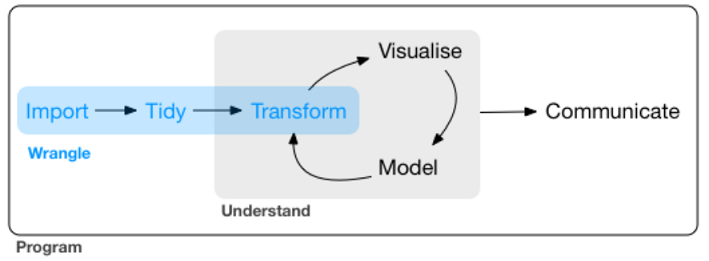
\includegraphics{image/wrangling.png}
\caption{\emph{Рис. 1. Структура задачі маніпулювання даними у складі Data Science-проекту}}
\end{figure}

\hypertarget{ux456ux43cux43fux43eux440ux442-ux434ux430ux43dux438ux445}{%
\subsection{Імпорт даних}\label{ux456ux43cux43fux43eux440ux442-ux434ux430ux43dux438ux445}}

Перша задача \emph{імпорту даних} (\textbf{Import}) полягає у вилученні необхідних сирих даних з будь-яких джерел (файли, БД, дані з датчиків у реальному часі і т. ін.) самого різного формату.\\
Вхідні дані можуть бути у трьох наступних форматах (прийнято також називати \emph{табульованими} (\textbf{Tabular Data}) і \emph{нетабульованими} (\textbf{Non-Tabular Data})):

\begin{itemize}
\tightlist
\item
  \emph{структурованому} -- у вигляді таблиці з чітко визначеними полями;
\item
  \emph{слабоструктурованому} -- так звані транзакційні дані, в яких проглядається певна структура, але немає чітко визначених полів та їх типів;\\
\item
  \emph{неструктурованому} -- будь-якому форматі, як правило, це текст довільної структури.
\end{itemize}

Для імпорту і експорту структурованих даних у середовищі R існує маса інструментів як стандартних, так і у складі спеціалізованих пакетів. Найпростіший варіант, який рекомендується для новачка, -- відповідні функції пакету \texttt{rio} \citep{rio}, що використовувався у лаб. ро. №1.

\begin{Shaded}
\begin{Highlighting}[]
\CommentTok{\# install\_formats() \#інсталяція додаткових компонентів пакету rio}
\FunctionTok{library}\NormalTok{(rio)}
\NormalTok{df }\OtherTok{\textless{}{-}} \FunctionTok{data.frame}\NormalTok{(}\AttributeTok{x =} \DecValTok{1}\SpecialCharTok{:}\DecValTok{5}\NormalTok{, }\AttributeTok{y =} \FunctionTok{rnorm}\NormalTok{(}\DecValTok{5}\NormalTok{))}
\FunctionTok{export}\NormalTok{(df, }\StringTok{"data/df\_data\_frame.txt"}\NormalTok{)}
\NormalTok{dfImp }\OtherTok{\textless{}{-}} \FunctionTok{import}\NormalTok{(}\StringTok{"data/df\_data\_frame.txt"}\NormalTok{)}
\NormalTok{dfImp}
\end{Highlighting}
\end{Shaded}

\begin{verbatim}
##   x          y
## 1 1  0.3157619
## 2 2  0.1347196
## 3 3  1.3754750
## 4 4  0.1256512
## 5 5 -0.8368388
\end{verbatim}

Пакет працює з файлами широкого спектру форматів і дозволяє виконувати за необхідності конвертацію файлів з одного формату в інший.

\begin{Shaded}
\begin{Highlighting}[]
\FunctionTok{data}\NormalTok{(}\StringTok{"mtcars"}\NormalTok{) }\CommentTok{\#підключення стандартного набору даних mtcars}
\CommentTok{\# head(mtcars)}
\FunctionTok{export}\NormalTok{(}\FunctionTok{head}\NormalTok{(mtcars), }\StringTok{"data/mtcars.dta"}\NormalTok{)}
\FunctionTok{convert}\NormalTok{(}\StringTok{\textquotesingle{}data/mtcars.dta\textquotesingle{}}\NormalTok{, }\StringTok{\textquotesingle{}data/mtcars.csv\textquotesingle{}}\NormalTok{)}
\FunctionTok{import}\NormalTok{(}\StringTok{"data/mtcars.csv"}\NormalTok{)}
\end{Highlighting}
\end{Shaded}

\begin{verbatim}
##    mpg cyl disp  hp drat    wt  qsec vs am gear carb
## 1 21.0   6  160 110 3.90 2.620 16.46  0  1    4    4
## 2 21.0   6  160 110 3.90 2.875 17.02  0  1    4    4
## 3 22.8   4  108  93 3.85 2.320 18.61  1  1    4    1
## 4 21.4   6  258 110 3.08 3.215 19.44  1  0    3    1
## 5 18.7   8  360 175 3.15 3.440 17.02  0  0    3    2
## 6 18.1   6  225 105 2.76 3.460 20.22  1  0    3    1
\end{verbatim}

\hypertarget{ux456ux43cux43fux43eux440ux442-ux437-ux440ux435ux43bux44fux446ux456ux439ux43dux438ux445-ux431ux430ux437-ux434ux430ux43dux438ux445}{%
\subsubsection{Імпорт з реляційних баз даних}\label{ux456ux43cux43fux43eux440ux442-ux437-ux440ux435ux43bux44fux446ux456ux439ux43dux438ux445-ux431ux430ux437-ux434ux430ux43dux438ux445}}

Пакет \citep{R-dplyr} забезпечує зручний інтерфейс дял роботи з віддаленими реляційними базами даних. Наразі ці можливості відокремлені в окремий пакет \href{https://cran.rstudio.com/web/packages/dbplyr/vignettes/dbplyr.html}{\texttt{dbplyr}} \citep{R-dbplyr}.
Основна перевага -- користувач повністю абстрагується від факту роботи з базою даних, оперуючи тими ж самими командами, що і для роботи з \texttt{data.frame} (див. нижче). \texttt{dbplyr} бере на себе повну відповідальність за роботу з БД, включаючи трансляцію команд на SQL. Хоча, в окремих випадках більш ефективно використовувати безпосередньо SQL!\\
Для роботи з \texttt{dbplyr} необхідно встановити пакет бекенда DBI. Пакет DBI забезпечує загальний інтерфейс, що дозволяє \texttt{dbplyr} працювати з багатьма різними базами даних, використовуючи один і той же код. DBI автоматично встановлюється за допомогою \texttt{dbplyr}, але необхідно окремо встановити конкретний бекенд для бази даних, до якої ми хочемо підключитися:

\begin{itemize}
\tightlist
\item
  \texttt{RMySQL} \citep{R-RMySQL} підключається до \texttt{MySQL} та \texttt{MariaDB};
\item
  \texttt{RPostgreSQL} \citep{R-RPostgreSQL} підключається до \texttt{Postgres} та \texttt{Redshift};
\item
  \texttt{RSQLite} \citep{R-RSQLite} вбудовує \texttt{SQLite}-базу даних;
\item
  \texttt{odbc} \citep{R-odbc} підключається до багатьох комерційних баз даних через протокол відкритої бази даних;
\item
  \texttt{bigrquery} \citep{R-bigrquery} підключається до \texttt{Google\ BigQuery}.
\end{itemize}

Для експериментів з базами даних найпростіше почати з \texttt{SQLite}, оскільки все необхідне включено в стандартний пакет \texttt{R}. Вам не потрібно встановлювати що-небудь ще і мати справу з налаштуванням сервера бази даних. Використовувати базу даних \texttt{SQLite} в \texttt{dplyr} дуже просто: достатньо задати шлях і відзначити, що потрібно створити нову БД:

\begin{Shaded}
\begin{Highlighting}[]
\FunctionTok{library}\NormalTok{(dbplyr)}
\FunctionTok{library}\NormalTok{(dplyr)}
\FunctionTok{library}\NormalTok{(RSQLite)}
\end{Highlighting}
\end{Shaded}

\begin{Shaded}
\begin{Highlighting}[]
\CommentTok{\# my\_db \textless{}{-} src\_sqlite("data/my\_db.sqlite3", create = T)}
\end{Highlighting}
\end{Shaded}

\texttt{my\_db} зараз не містить даних, тому ми завантажимо туди дані \texttt{flights} (зі стандартного набору \citep{R-nycflights13}) з використанням зручної функції \texttt{copy\_to()}. Це швидкий і ``брудний'' спосіб для того, щоб помістити дані в базу даних, але він не підходить для дуже великих наборів даних, оскільки всі дані повинні проходити через \texttt{R}.

\begin{Shaded}
\begin{Highlighting}[]
\FunctionTok{library}\NormalTok{(nycflights13)}
\CommentTok{\# flights\_sqlite \textless{}{-} copy\_to(my\_db, flights, temporary = FALSE, }
\CommentTok{\#                           indexes = list(c("year", "month", "day"), "carrier", "tailnum"))}
\CommentTok{\# head(flights\_sqlite)}
\end{Highlighting}
\end{Shaded}

Нижче показано приклад встановлення з'єднання з існуючою БД через функцію \texttt{DBConnect}, що входить до складу \texttt{DBI} \citep{R-DBI}.

\begin{Shaded}
\begin{Highlighting}[]
\NormalTok{con }\OtherTok{\textless{}{-}}\NormalTok{ DBI}\SpecialCharTok{::}\FunctionTok{dbConnect}\NormalTok{(RSQLite}\SpecialCharTok{::}\FunctionTok{SQLite}\NormalTok{(), }\AttributeTok{path =} \StringTok{"data/my\_db.sqlite3"}\NormalTok{)}
\NormalTok{flights\_sqlite }\OtherTok{\textless{}{-}} \FunctionTok{copy\_to}\NormalTok{(con, nycflights13}\SpecialCharTok{::}\NormalTok{flights, }\StringTok{"flights"}\NormalTok{,}
        \AttributeTok{temporary =} \ConstantTok{FALSE}\NormalTok{, }
        \AttributeTok{indexes =} \FunctionTok{list}\NormalTok{(}
          \FunctionTok{c}\NormalTok{(}\StringTok{"year"}\NormalTok{, }\StringTok{"month"}\NormalTok{, }\StringTok{"day"}\NormalTok{), }
          \StringTok{"carrier"}\NormalTok{, }
          \StringTok{"tailnum"}\NormalTok{,}
          \StringTok{"dest"}
\NormalTok{        )}
\NormalTok{)}

\FunctionTok{head}\NormalTok{(flights\_sqlite)}
\end{Highlighting}
\end{Shaded}

\begin{verbatim}
## # Source:   lazy query [?? x 19]
## # Database: sqlite 3.37.2 []
##    year month   day dep_time sched_dep_time dep_delay arr_time sched_arr_time
##   <int> <int> <int>    <int>          <int>     <dbl>    <int>          <int>
## 1  2013     1     1      517            515         2      830            819
## 2  2013     1     1      533            529         4      850            830
## 3  2013     1     1      542            540         2      923            850
## 4  2013     1     1      544            545        -1     1004           1022
## 5  2013     1     1      554            600        -6      812            837
## 6  2013     1     1      554            558        -4      740            728
## # ... with 11 more variables: arr_delay <dbl>, carrier <chr>, flight <int>,
## #   tailnum <chr>, origin <chr>, dest <chr>, air_time <dbl>, distance <dbl>,
## #   hour <dbl>, minute <dbl>, time_hour <dbl>
\end{verbatim}

Для більш детального знайомства доцільно скористатися вищезаначеними посиланнями, та матеріалами \href{https://db.rstudio.com/dplyr/}{проекту RStudio} \citep{R-dbplyr}, присвяченого роботі з БД в середовищі \texttt{RStudio}, а також \href{http://biostat-r.blogspot.com/2015/07/dplyr-databases.html\#more}{російськомовним перекладом Андрія Огурцова} документації по \texttt{dplyr}.

При роботі зі слабоструктурованими та неструктурованими файлами, або коли необхідно маніпулювати даними вже на етапі імпорту, можна скористатися потужностями пакету \citep{R-reader} для парсингу даних з нетабульованих джерел за допомогою сімейства методів \texttt{read\_*}, \texttt{col\_*}, \texttt{parse\_*}, включаючи рядки (\textbf{strings}), категоріальні змінні (\textbf{factors}), данні типу час-дата (\textbf{data-time}) (див. шпаргалку \href{doc/data-import.pdf}{тут}), що входить до колекції \href{https://www.tidyverse.org/}{tidyvers}.

\hypertarget{ux43fux440ux438ux432ux435ux434ux435ux43dux43dux44f-ux434ux430ux43dux438ux445-ux434ux43e-ux43eux445ux430ux439ux43dux43eux433ux43e-ux432ux438ux433ux43bux44fux434ux443}{%
\subsection{Приведення даних до охайного вигляду}\label{ux43fux440ux438ux432ux435ux434ux435ux43dux43dux44f-ux434ux430ux43dux438ux445-ux434ux43e-ux43eux445ux430ux439ux43dux43eux433ux43e-ux432ux438ux433ux43bux44fux434ux443}}

\hypertarget{ux449ux43e-ux442ux430ux43aux435-ux43eux445ux430ux439ux43dux456-ux434ux430ux43dux456-tidy-data}{%
\subsubsection{Що таке ``охайні дані (tidy data)?}\label{ux449ux43e-ux442ux430ux43aux435-ux43eux445ux430ux439ux43dux456-ux434ux430ux43dux456-tidy-data}}

Друга і найбільш трудомістка задача (\textbf{Tidy}) -- \emph{приведення даних до} так званого \emph{``охайного'' вигляду}, придатного для аналізу. Як правило мова йде про приведення даних до табличного вигляду ``ключ-значення'', або, іншими словами, ``об'єкт-ознака''.\\
Колекція \texttt{tidyvers} будує сво роботу навколо ``охайних'' даних, збережених у так званих \texttt{tibbles}, що є розширенням типу \texttt{data.frame}. Забезпечується це за допомогою пакету \texttt{tibble}, який предоставляє новий S3 клас для збереження табличних даних. \texttt{tibbles} наслідує клас \texttt{data.frame} і покращує деякі маніпулятивні процедури (див. шпаргалку \href{doc/data-import.pdf}{тут}).\\
Розглянемо інструментарій пакету \href{https://cran.r-project.org/web/packages/tidyr/tidyr.pdf}{tidyr}, який вхродить до складу \texttt{tidyvers}, використовуючи матеріали з книги \citep{r4ds}. (Більш детально -- див. статтю \citep{tidy}, або \href{http://biostat-r.blogspot.com/2016/01/tidy-data.html\#more}{скорочений переклад російською}).\\
Існує три взаємопов'язані правила, які роблять набір даних ``охайним'':

\begin{itemize}
\tightlist
\item
  Кожна змінна містится у окремому полі;
\item
  Кожне спостереження має містится у окремому рядку;
\item
  Значення кожної змінної має міститися в окремій комірці.
\end{itemize}

\begin{figure}
\centering
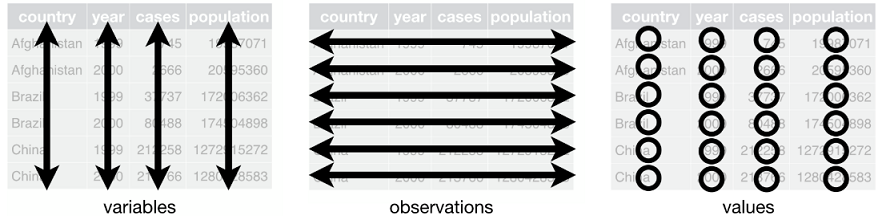
\includegraphics{image/tidy.png}
\caption{\emph{Рис. 2. Три взаємопов'язані правила, які роблять набір даних ``охайними''}}
\end{figure}

Чому доцільно приводити дані до охайного виду? В цьому є дві переваги:

\begin{itemize}
\tightlist
\item
  загальна перевага -- такого роду уніфікований вид даних дозволяє ефективно їх зберігати, в тому числі, у реляційній базі даних, і дозволяє маніпулювати їми за допомогою стандартних інструментів;
\item
  специфічна перевага -- мова R з точки зору написання ефективного коду передбачає виконання процедури векторизації у всіх випадках, коли це можливо, а це потребує приведення коду до охайного вигляду.
\end{itemize}

Нижче наведено приклад роботи з таблицею, що має охайний вигляд.

\begin{Shaded}
\begin{Highlighting}[]
\FunctionTok{library}\NormalTok{(tidyverse)}
\end{Highlighting}
\end{Shaded}

\begin{Shaded}
\begin{Highlighting}[]
\CommentTok{\# відносний критерій на 10000}
\NormalTok{table1 }\SpecialCharTok{\%\textgreater{}\%}  \CommentTok{\# стандартний набір даних}
  \FunctionTok{mutate}\NormalTok{(}\AttributeTok{rate =}\NormalTok{ cases }\SpecialCharTok{/}\NormalTok{ population }\SpecialCharTok{*} \DecValTok{10000}\NormalTok{) }\CommentTok{\# обчислення нового поля}
\end{Highlighting}
\end{Shaded}

\begin{verbatim}
## # A tibble: 6 x 5
##   country      year  cases population  rate
##   <chr>       <int>  <int>      <int> <dbl>
## 1 Afghanistan  1999    745   19987071 0.373
## 2 Afghanistan  2000   2666   20595360 1.29 
## 3 Brazil       1999  37737  172006362 2.19 
## 4 Brazil       2000  80488  174504898 4.61 
## 5 China        1999 212258 1272915272 1.67 
## 6 China        2000 213766 1280428583 1.67
\end{verbatim}

\begin{Shaded}
\begin{Highlighting}[]
\CommentTok{\# кількість випадків на рік}
\NormalTok{table1 }\SpecialCharTok{\%\textgreater{}\%} 
  \FunctionTok{count}\NormalTok{(year, }\AttributeTok{wt =}\NormalTok{ cases)}
\end{Highlighting}
\end{Shaded}

\begin{verbatim}
## # A tibble: 2 x 2
##    year      n
##   <int>  <int>
## 1  1999 250740
## 2  2000 296920
\end{verbatim}

Потоковий оператор \texttt{\%\textgreater{}\%} дає можливість спрощувати написання коду. Оператор працює наступним чином: вираз \texttt{sin(cos(x))} може бути переписаний як \texttt{x\ \%\textgreater{}\%\ cos()\ \%\textgreater{}\%\ sin()}.

Нижче наведено приклад сумісного застосування потокового оператору і функцій пакету {[}R-ggplot2{]} для візуалізації результатів.

\begin{Shaded}
\begin{Highlighting}[]
\CommentTok{\# Візуалізація динаміки зміни кількості випадків з часом}
\FunctionTok{library}\NormalTok{(ggplot2)}
\FunctionTok{ggplot}\NormalTok{(table1, }\FunctionTok{aes}\NormalTok{(year, cases)) }\SpecialCharTok{+} 
  \FunctionTok{geom\_line}\NormalTok{(}\FunctionTok{aes}\NormalTok{(}\AttributeTok{group =}\NormalTok{ country), }\AttributeTok{colour =} \StringTok{"grey50"}\NormalTok{) }\SpecialCharTok{+} 
  \FunctionTok{geom\_point}\NormalTok{(}\FunctionTok{aes}\NormalTok{(}\AttributeTok{colour =}\NormalTok{ country))}
\end{Highlighting}
\end{Shaded}

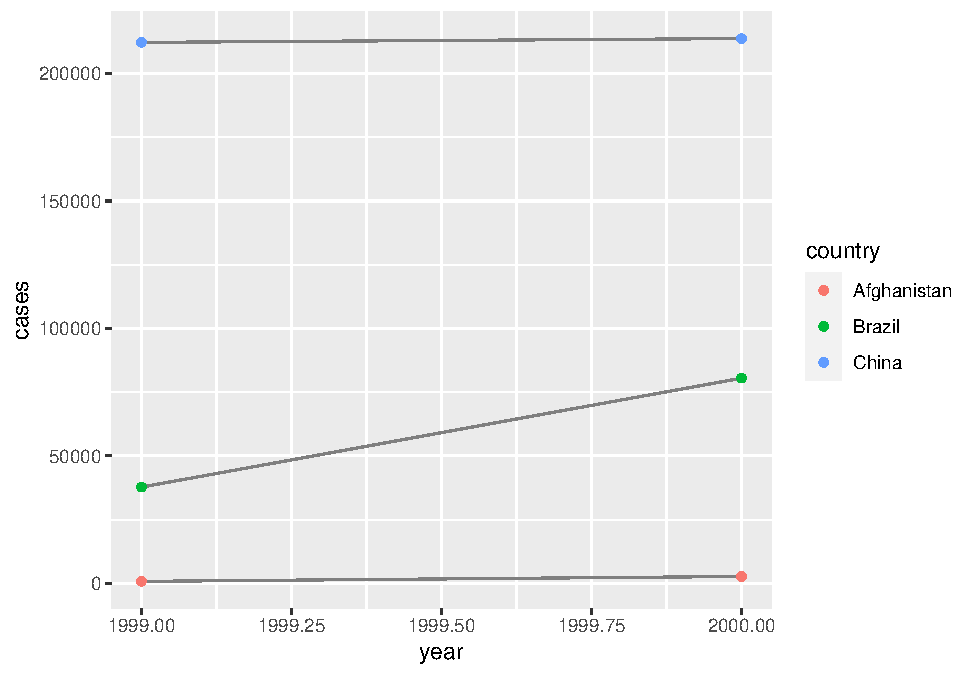
\includegraphics{DS-book-lab_files/figure-latex/unnamed-chunk-11-1.pdf}

\begin{Shaded}
\begin{Highlighting}[]
\CommentTok{\# table1 \%\textgreater{}\% }
\CommentTok{\#   mutate(rate = cases / population * 10000) \%\textgreater{}\% }
\CommentTok{\#   ggplot(aes(year, rate)) + }
\CommentTok{\#   geom\_line(aes(group = country), colour = "grey50") + }
\CommentTok{\#   geom\_point(aes(colour = country))}
\end{Highlighting}
\end{Shaded}

\textbf{Завдання на самостійну роботу}. Побудувати динаміку відносного критерію \texttt{rate} кількості захворювань по роках для кожної держави.

\hypertarget{ux43fux440ux43eux446ux435ux434ux443ux440ux438-spreading-and-gathering}{%
\subsubsection{Процедури Spreading and Gathering}\label{ux43fux440ux43eux446ux435ux434ux443ux440ux438-spreading-and-gathering}}

На практиці найбільш часто зустрічаються два основних типи ``неохайності'' даних:

\begin{itemize}
\tightlist
\item
  Значення однієї змінної можуть бути розкидані по багатьох стовпчиках;
\item
  Одне спостереження може бути розсіяне по багатьох рядках.
\end{itemize}

Для вирішення цієї проблеми у складі пакету \texttt{tidyr} існують функції \texttt{gather()}і \texttt{spread()}.

\hypertarget{gathering}{%
\paragraph{Gathering}\label{gathering}}

Поширеною проблемою є набір даних, де деякі назви стовпців -- це не імена змінних, а значення змінної. Візьміть table4a: назви стовпчиків 1999 та 2000 представляють значення змінної року, і кожен рядок містить два спостереження, а не одне.

\begin{Shaded}
\begin{Highlighting}[]
\NormalTok{table4a}
\end{Highlighting}
\end{Shaded}

\begin{verbatim}
## # A tibble: 3 x 3
##   country     `1999` `2000`
## * <chr>        <int>  <int>
## 1 Afghanistan    745   2666
## 2 Brazil       37737  80488
## 3 China       212258 213766
\end{verbatim}

Для розв'язку проблеми необхідно зібрати (\textbf{gather}) необхідні колонки у пару нових змінних (рис. 3).

\begin{figure}
\centering
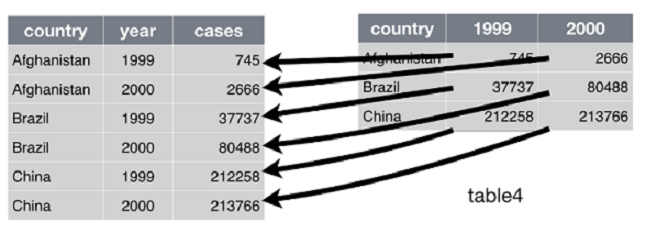
\includegraphics{image/table4.png}
\caption{\emph{Рис. 3 Приведення \texttt{table4} до охайної форми}}
\end{figure}

\begin{Shaded}
\begin{Highlighting}[]
\NormalTok{table4a }\SpecialCharTok{\%\textgreater{}\%} 
  \FunctionTok{gather}\NormalTok{(}\StringTok{\textasciigrave{}}\AttributeTok{1999}\StringTok{\textasciigrave{}}\NormalTok{, }\StringTok{\textasciigrave{}}\AttributeTok{2000}\StringTok{\textasciigrave{}}\NormalTok{, }\AttributeTok{key =} \StringTok{"year"}\NormalTok{, }\AttributeTok{value =} \StringTok{"cases"}\NormalTok{)}
\end{Highlighting}
\end{Shaded}

\begin{verbatim}
## # A tibble: 6 x 3
##   country     year   cases
##   <chr>       <chr>  <int>
## 1 Afghanistan 1999     745
## 2 Brazil      1999   37737
## 3 China       1999  212258
## 4 Afghanistan 2000    2666
## 5 Brazil      2000   80488
## 6 China       2000  213766
\end{verbatim}

Для комбінування таблиць після приведення їх до охайного вигляду, можна використовувати ліве з'єднання.

\begin{Shaded}
\begin{Highlighting}[]
\NormalTok{tidy4a }\OtherTok{\textless{}{-}}\NormalTok{ table4a }\SpecialCharTok{\%\textgreater{}\%} 
  \FunctionTok{gather}\NormalTok{(}\StringTok{\textasciigrave{}}\AttributeTok{1999}\StringTok{\textasciigrave{}}\NormalTok{, }\StringTok{\textasciigrave{}}\AttributeTok{2000}\StringTok{\textasciigrave{}}\NormalTok{, }\AttributeTok{key =} \StringTok{"year"}\NormalTok{, }\AttributeTok{value =} \StringTok{"cases"}\NormalTok{)}
\NormalTok{tidy4b }\OtherTok{\textless{}{-}}\NormalTok{ table4b }\SpecialCharTok{\%\textgreater{}\%} 
  \FunctionTok{gather}\NormalTok{(}\StringTok{\textasciigrave{}}\AttributeTok{1999}\StringTok{\textasciigrave{}}\NormalTok{, }\StringTok{\textasciigrave{}}\AttributeTok{2000}\StringTok{\textasciigrave{}}\NormalTok{, }\AttributeTok{key =} \StringTok{"year"}\NormalTok{, }\AttributeTok{value =} \StringTok{"population"}\NormalTok{)}
\NormalTok{dplyr}\SpecialCharTok{::}\FunctionTok{left\_join}\NormalTok{(tidy4a, tidy4b)}
\end{Highlighting}
\end{Shaded}

\begin{verbatim}
## Joining, by = c("country", "year")
\end{verbatim}

\begin{verbatim}
## # A tibble: 6 x 4
##   country     year   cases population
##   <chr>       <chr>  <int>      <int>
## 1 Afghanistan 1999     745   19987071
## 2 Brazil      1999   37737  172006362
## 3 China       1999  212258 1272915272
## 4 Afghanistan 2000    2666   20595360
## 5 Brazil      2000   80488  174504898
## 6 China       2000  213766 1280428583
\end{verbatim}

\textbf{Завдання на самостійну роботу}. Виконати попереднє завдання, базуючись на таблицях \texttt{tidy4a} і \texttt{tidy4b} з використанням потокового оператора.

\hypertarget{spreading}{%
\paragraph{Spreading}\label{spreading}}

Це процедура протилежна збиранню. Поширення, або розтягування (spreading) застосовується, коли спостереження знаходяться в різних рядках (рис. 4).

\begin{figure}
\centering
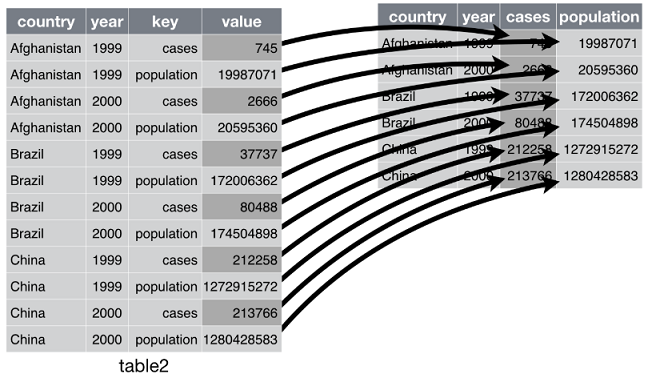
\includegraphics{image/table2.png}
\caption{\emph{Рис. 4 Приведення \texttt{table2} до охайної форми}}
\end{figure}

Приклад.

\begin{Shaded}
\begin{Highlighting}[]
\NormalTok{table2}
\end{Highlighting}
\end{Shaded}

\begin{verbatim}
## # A tibble: 12 x 4
##    country      year type            count
##    <chr>       <int> <chr>           <int>
##  1 Afghanistan  1999 cases             745
##  2 Afghanistan  1999 population   19987071
##  3 Afghanistan  2000 cases            2666
##  4 Afghanistan  2000 population   20595360
##  5 Brazil       1999 cases           37737
##  6 Brazil       1999 population  172006362
##  7 Brazil       2000 cases           80488
##  8 Brazil       2000 population  174504898
##  9 China        1999 cases          212258
## 10 China        1999 population 1272915272
## 11 China        2000 cases          213766
## 12 China        2000 population 1280428583
\end{verbatim}

\begin{Shaded}
\begin{Highlighting}[]
\NormalTok{table2 }\SpecialCharTok{\%\textgreater{}\%}
    \FunctionTok{spread}\NormalTok{(}\AttributeTok{key =}\NormalTok{ type, }\AttributeTok{value =}\NormalTok{ count)}
\end{Highlighting}
\end{Shaded}

\begin{verbatim}
## # A tibble: 6 x 4
##   country      year  cases population
##   <chr>       <int>  <int>      <int>
## 1 Afghanistan  1999    745   19987071
## 2 Afghanistan  2000   2666   20595360
## 3 Brazil       1999  37737  172006362
## 4 Brazil       2000  80488  174504898
## 5 China        1999 212258 1272915272
## 6 China        2000 213766 1280428583
\end{verbatim}

\hypertarget{ux43fux440ux43eux446ux435ux434ux443ux440ux438-separating-ux456-uniting}{%
\subsubsection{Процедури Separating і Uniting}\label{ux43fux440ux43eux446ux435ux434ux443ux440ux438-separating-ux456-uniting}}

На практиці може статися випадок, коли в одному стовпчику знаходяться різні змінні. Проблема вирішується шляхом його розділення (separating) на два (див. рис.5).

\begin{figure}
\centering
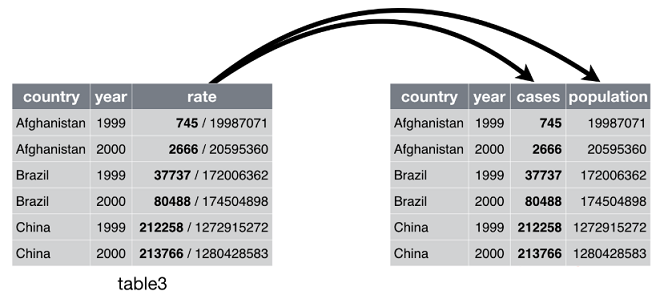
\includegraphics{image/table3.png}
\caption{\emph{Рис. 5 Приведення \texttt{table3} до охайної форми шляхом розділення стовпчиків}}
\end{figure}

\begin{Shaded}
\begin{Highlighting}[]
\NormalTok{table3}
\end{Highlighting}
\end{Shaded}

\begin{verbatim}
## # A tibble: 6 x 3
##   country      year rate             
## * <chr>       <int> <chr>            
## 1 Afghanistan  1999 745/19987071     
## 2 Afghanistan  2000 2666/20595360    
## 3 Brazil       1999 37737/172006362  
## 4 Brazil       2000 80488/174504898  
## 5 China        1999 212258/1272915272
## 6 China        2000 213766/1280428583
\end{verbatim}

\begin{Shaded}
\begin{Highlighting}[]
\NormalTok{table3 }\SpecialCharTok{\%\textgreater{}\%} 
  \FunctionTok{separate}\NormalTok{(rate, }\AttributeTok{into =} \FunctionTok{c}\NormalTok{(}\StringTok{"cases"}\NormalTok{, }\StringTok{"population"}\NormalTok{))}
\end{Highlighting}
\end{Shaded}

\begin{verbatim}
## # A tibble: 6 x 4
##   country      year cases  population
##   <chr>       <int> <chr>  <chr>     
## 1 Afghanistan  1999 745    19987071  
## 2 Afghanistan  2000 2666   20595360  
## 3 Brazil       1999 37737  172006362 
## 4 Brazil       2000 80488  174504898 
## 5 China        1999 212258 1272915272
## 6 China        2000 213766 1280428583
\end{verbatim}

Зворотною процедурою до \texttt{separate()} є \texttt{unite()}.

\begin{Shaded}
\begin{Highlighting}[]
\NormalTok{table5 }\SpecialCharTok{\%\textgreater{}\%} 
  \FunctionTok{unite}\NormalTok{(new, century, year, }\AttributeTok{sep =} \StringTok{""}\NormalTok{)}
\end{Highlighting}
\end{Shaded}

\begin{verbatim}
## # A tibble: 6 x 3
##   country     new   rate             
##   <chr>       <chr> <chr>            
## 1 Afghanistan 1999  745/19987071     
## 2 Afghanistan 2000  2666/20595360    
## 3 Brazil      1999  37737/172006362  
## 4 Brazil      2000  80488/174504898  
## 5 China       1999  212258/1272915272
## 6 China       2000  213766/1280428583
\end{verbatim}

\hypertarget{ux43fux440ux43eux43fux443ux449ux435ux43dux456-ux437ux43dux430ux447ux435ux43dux43dux44f}{%
\subsubsection{Пропущені значення}\label{ux43fux440ux43eux43fux443ux449ux435ux43dux456-ux437ux43dux430ux447ux435ux43dux43dux44f}}

Пропущені значення (\textbf{missing value}) у наборах даних можуть бути двох видів: \emph{явні} (позначені як \texttt{NA}, \texttt{Not\ Available}) і \emph{неявні} (просто не представлені у даних). Такі дані називаються \emph{некомплектні}.\\
Нижче наведено приклад, який це ілюструє.

\begin{Shaded}
\begin{Highlighting}[]
\NormalTok{stocks }\OtherTok{\textless{}{-}} \FunctionTok{tibble}\NormalTok{(}
  \AttributeTok{year   =} \FunctionTok{c}\NormalTok{(}\DecValTok{2015}\NormalTok{, }\DecValTok{2015}\NormalTok{, }\DecValTok{2015}\NormalTok{, }\DecValTok{2015}\NormalTok{, }\DecValTok{2016}\NormalTok{, }\DecValTok{2016}\NormalTok{, }\DecValTok{2016}\NormalTok{),}
  \AttributeTok{qtr    =} \FunctionTok{c}\NormalTok{(   }\DecValTok{1}\NormalTok{,    }\DecValTok{2}\NormalTok{,    }\DecValTok{3}\NormalTok{,    }\DecValTok{4}\NormalTok{,    }\DecValTok{2}\NormalTok{,    }\DecValTok{3}\NormalTok{,    }\DecValTok{4}\NormalTok{),}
  \AttributeTok{return =} \FunctionTok{c}\NormalTok{(}\FloatTok{1.88}\NormalTok{, }\FloatTok{0.59}\NormalTok{, }\FloatTok{0.35}\NormalTok{,   }\ConstantTok{NA}\NormalTok{, }\FloatTok{0.92}\NormalTok{, }\FloatTok{0.17}\NormalTok{, }\FloatTok{2.66}\NormalTok{)}
\NormalTok{)}
\NormalTok{stocks}
\end{Highlighting}
\end{Shaded}

\begin{verbatim}
## # A tibble: 7 x 3
##    year   qtr return
##   <dbl> <dbl>  <dbl>
## 1  2015     1   1.88
## 2  2015     2   0.59
## 3  2015     3   0.35
## 4  2015     4  NA   
## 5  2016     2   0.92
## 6  2016     3   0.17
## 7  2016     4   2.66
\end{verbatim}

Дані за четвертий квартал 2015 явно відсутні про що свідчить відповідне значення. Дані за перший квартал не внесені у таблицю, тобто відсутні неявно, але відсутність можна помітити після відповідної траснформації.

\begin{Shaded}
\begin{Highlighting}[]
\NormalTok{stocks }\SpecialCharTok{\%\textgreater{}\%} 
  \FunctionTok{spread}\NormalTok{(year, return)}
\end{Highlighting}
\end{Shaded}

\begin{verbatim}
## # A tibble: 4 x 3
##     qtr `2015` `2016`
##   <dbl>  <dbl>  <dbl>
## 1     1   1.88  NA   
## 2     2   0.59   0.92
## 3     3   0.35   0.17
## 4     4  NA      2.66
\end{verbatim}

Виявити множину некомплектних даних можна також з використанням функції \texttt{complete()}.

\begin{Shaded}
\begin{Highlighting}[]
\NormalTok{stocks }\SpecialCharTok{\%\textgreater{}\%} 
  \FunctionTok{complete}\NormalTok{(year, qtr)}
\end{Highlighting}
\end{Shaded}

\begin{verbatim}
## # A tibble: 8 x 3
##    year   qtr return
##   <dbl> <dbl>  <dbl>
## 1  2015     1   1.88
## 2  2015     2   0.59
## 3  2015     3   0.35
## 4  2015     4  NA   
## 5  2016     1  NA   
## 6  2016     2   0.92
## 7  2016     3   0.17
## 8  2016     4   2.66
\end{verbatim}

Проблема некомплектних даних вирішується двома шляхами: виключенням некомплектних спостережень, або імпутацією пропущених значень іншими значеннями, виходячи з певної моделі.

\begin{Shaded}
\begin{Highlighting}[]
\NormalTok{stocks }\SpecialCharTok{\%\textgreater{}\%} 
  \FunctionTok{spread}\NormalTok{(year, return) }\SpecialCharTok{\%\textgreater{}\%} 
  \FunctionTok{gather}\NormalTok{(year, return, }\StringTok{\textasciigrave{}}\AttributeTok{2015}\StringTok{\textasciigrave{}}\SpecialCharTok{:}\StringTok{\textasciigrave{}}\AttributeTok{2016}\StringTok{\textasciigrave{}}\NormalTok{, }\AttributeTok{na.rm =} \ConstantTok{TRUE}\NormalTok{)}
\end{Highlighting}
\end{Shaded}

\begin{verbatim}
## # A tibble: 6 x 3
##     qtr year  return
##   <dbl> <chr>  <dbl>
## 1     1 2015    1.88
## 2     2 2015    0.59
## 3     3 2015    0.35
## 4     2 2016    0.92
## 5     3 2016    0.17
## 6     4 2016    2.66
\end{verbatim}

У випадках, коли це доцільно, можна використовувати функцію \texttt{fill()}, яка заповнює пропущенні значення, взявши значення з останньої заповненої клітинки:

\begin{Shaded}
\begin{Highlighting}[]
\NormalTok{df }\OtherTok{\textless{}{-}} \FunctionTok{data.frame}\NormalTok{(}\AttributeTok{Month =} \DecValTok{1}\SpecialCharTok{:}\DecValTok{12}\NormalTok{, }\AttributeTok{Year =} \FunctionTok{c}\NormalTok{(}\DecValTok{2000}\NormalTok{, }\FunctionTok{rep}\NormalTok{(}\ConstantTok{NA}\NormalTok{, }\DecValTok{11}\NormalTok{)))}
\NormalTok{df}
\end{Highlighting}
\end{Shaded}

\begin{verbatim}
##    Month Year
## 1      1 2000
## 2      2   NA
## 3      3   NA
## 4      4   NA
## 5      5   NA
## 6      6   NA
## 7      7   NA
## 8      8   NA
## 9      9   NA
## 10    10   NA
## 11    11   NA
## 12    12   NA
\end{verbatim}

\begin{Shaded}
\begin{Highlighting}[]
\NormalTok{df }\SpecialCharTok{\%\textgreater{}\%} \FunctionTok{fill}\NormalTok{(Year)}
\end{Highlighting}
\end{Shaded}

\begin{verbatim}
##    Month Year
## 1      1 2000
## 2      2 2000
## 3      3 2000
## 4      4 2000
## 5      5 2000
## 6      6 2000
## 7      7 2000
## 8      8 2000
## 9      9 2000
## 10    10 2000
## 11    11 2000
## 12    12 2000
\end{verbatim}

\hypertarget{ux442ux440ux430ux43dux441ux444ux43eux440ux43cux430ux446ux456ux44f}{%
\subsection{Трансформація}\label{ux442ux440ux430ux43dux441ux444ux43eux440ux43cux430ux446ux456ux44f}}

Недостатньо привести дані до охайного вигляду. Найбільш важливі процедури візуалізації та моделювання потребують різного роду трасформації охайних даних: вибірки рядків та полів, перейменування та зміну типів даних, обчислення нових значень, різного роду агрегації тощо.
\textbf{Трансформація} (\textbf{Transform}) -- друга важлива задача у складі процедури маніпулювання даними.\\
Середовище R наразі має низку потужних інструментів для цього, які побудовані на схожих концепціях, серед яких одним з найбільш поширених і потужних є пакет \href{https://cran.r-project.org/web/packages/dplyr/}{dplyr} \citep{dplyr} зі своєю, як прийнято говорити у професійних колах, ``філософією''.\\
Наведемо короткий огляд основих команд і прикладів їх застосування згідно з \citep{tvdplyr}.\\
Як стверджують розробники, \texttt{dplyr} -- граматика маніпулювання даними, що забезпечує послідовний набір дієслів, які допомагають вирішити найбільш поширені проблеми з обробкою даних:

\begin{itemize}
\tightlist
\item
  \texttt{mutate()} додає нові змінні, які є функціями існуючих змінних.
\item
  \texttt{select()} вибирає стовпчики (поля таблиці) на основі їх імен.
\item
  \texttt{filter()} вибирає рядки (спостереження) на основі їх значень.
\item
  \texttt{summarise()} зменшує декілька значень до одного резюме.
\item
  \texttt{arrange()} змінює упорядкування рядків.
\end{itemize}

Усі ці команди об'єднуються природним чином з функцією групування \texttt{group\_by()}, яка дозволяє виконувати будь-яку операцію ``по групі''. Поряд з даними командами для одинарних таблиць \texttt{dplyr} також надає різноманітні команди для \href{https://dplyr.tidyverse.org/articles/two-table.html}{двох таблиць}. Для \href{http://adv-r.had.co.nz/Functionals.html\#functionals-fp}{маніпулювання багатьма таблицями} викорстовуються засоби пакету \href{https://purrr.tidyverse.org/}{\texttt{purrr}} в парадигмі функціонального програмування, який також входить до \texttt{tidyverse}.\\
Як було зазначено вище, \texttt{dplyr} розроблений для того, щоб абстрагуватися від форми, у якій зберігаються дані. Це означає, що при роботі з локальними таблицями даних і з віддаленими таблицями бази даних використовується один і той же самий код R.\\
Враховуючи, що більшість команд за своїм сенсом ідентична SQL-командам, з якими студент вже знайомий, наведемо коротко основні приклади їх застосування без зайвих коментарів.

\begin{Shaded}
\begin{Highlighting}[]
\CommentTok{\# Вибірка рядків таблиці}
\FunctionTok{library}\NormalTok{(dplyr)}

\NormalTok{starwars }\SpecialCharTok{\%\textgreater{}\%} 
  \FunctionTok{filter}\NormalTok{(species }\SpecialCharTok{==} \StringTok{"Droid"}\NormalTok{)}
\end{Highlighting}
\end{Shaded}

\begin{verbatim}
## # A tibble: 6 x 14
##   name   height  mass hair_color skin_color  eye_color birth_year sex   gender  
##   <chr>   <int> <dbl> <chr>      <chr>       <chr>          <dbl> <chr> <chr>   
## 1 C-3PO     167    75 <NA>       gold        yellow           112 none  masculi~
## 2 R2-D2      96    32 <NA>       white, blue red               33 none  masculi~
## 3 R5-D4      97    32 <NA>       white, red  red               NA none  masculi~
## 4 IG-88     200   140 none       metal       red               15 none  masculi~
## 5 R4-P17     96    NA none       silver, red red, blue         NA none  feminine
## 6 BB8        NA    NA none       none        black             NA none  masculi~
## # ... with 5 more variables: homeworld <chr>, species <chr>, films <list>,
## #   vehicles <list>, starships <list>
\end{verbatim}

\begin{Shaded}
\begin{Highlighting}[]
\CommentTok{\# Вибірка полів таблиці}
\NormalTok{starwars }\SpecialCharTok{\%\textgreater{}\%} 
  \FunctionTok{select}\NormalTok{(name, }\FunctionTok{ends\_with}\NormalTok{(}\StringTok{"color"}\NormalTok{))}
\end{Highlighting}
\end{Shaded}

\begin{verbatim}
## # A tibble: 87 x 4
##    name               hair_color    skin_color  eye_color
##    <chr>              <chr>         <chr>       <chr>    
##  1 Luke Skywalker     blond         fair        blue     
##  2 C-3PO              <NA>          gold        yellow   
##  3 R2-D2              <NA>          white, blue red      
##  4 Darth Vader        none          white       yellow   
##  5 Leia Organa        brown         light       brown    
##  6 Owen Lars          brown, grey   light       blue     
##  7 Beru Whitesun lars brown         light       blue     
##  8 R5-D4              <NA>          white, red  red      
##  9 Biggs Darklighter  black         light       brown    
## 10 Obi-Wan Kenobi     auburn, white fair        blue-gray
## # ... with 77 more rows
\end{verbatim}

\begin{Shaded}
\begin{Highlighting}[]
\CommentTok{\# Створення нового поля у таблиці з послідуючою вибіркою}
\NormalTok{starwars }\SpecialCharTok{\%\textgreater{}\%} 
  \FunctionTok{mutate}\NormalTok{(name, }\AttributeTok{bmi =}\NormalTok{ mass }\SpecialCharTok{/}\NormalTok{ ((height }\SpecialCharTok{/} \DecValTok{100}\NormalTok{)  }\SpecialCharTok{\^{}} \DecValTok{2}\NormalTok{)) }\SpecialCharTok{\%\textgreater{}\%}
  \FunctionTok{select}\NormalTok{(name}\SpecialCharTok{:}\NormalTok{mass, bmi)}
\end{Highlighting}
\end{Shaded}

\begin{verbatim}
## # A tibble: 87 x 4
##    name               height  mass   bmi
##    <chr>               <int> <dbl> <dbl>
##  1 Luke Skywalker        172    77  26.0
##  2 C-3PO                 167    75  26.9
##  3 R2-D2                  96    32  34.7
##  4 Darth Vader           202   136  33.3
##  5 Leia Organa           150    49  21.8
##  6 Owen Lars             178   120  37.9
##  7 Beru Whitesun lars    165    75  27.5
##  8 R5-D4                  97    32  34.0
##  9 Biggs Darklighter     183    84  25.1
## 10 Obi-Wan Kenobi        182    77  23.2
## # ... with 77 more rows
\end{verbatim}

\begin{Shaded}
\begin{Highlighting}[]
\CommentTok{\# Сортування даних}
\NormalTok{starwars }\SpecialCharTok{\%\textgreater{}\%} 
  \FunctionTok{arrange}\NormalTok{(}\FunctionTok{desc}\NormalTok{(mass))}
\end{Highlighting}
\end{Shaded}

\begin{verbatim}
## # A tibble: 87 x 14
##    name     height  mass hair_color skin_color eye_color birth_year sex   gender
##    <chr>     <int> <dbl> <chr>      <chr>      <chr>          <dbl> <chr> <chr> 
##  1 Jabba D~    175  1358 <NA>       green-tan~ orange         600   herm~ mascu~
##  2 Grievous    216   159 none       brown, wh~ green, y~       NA   male  mascu~
##  3 IG-88       200   140 none       metal      red             15   none  mascu~
##  4 Darth V~    202   136 none       white      yellow          41.9 male  mascu~
##  5 Tarfful     234   136 brown      brown      blue            NA   male  mascu~
##  6 Owen La~    178   120 brown, gr~ light      blue            52   male  mascu~
##  7 Bossk       190   113 none       green      red             53   male  mascu~
##  8 Chewbac~    228   112 brown      unknown    blue           200   male  mascu~
##  9 Jek Ton~    180   110 brown      fair       blue            NA   male  mascu~
## 10 Dexter ~    198   102 none       brown      yellow          NA   male  mascu~
## # ... with 77 more rows, and 5 more variables: homeworld <chr>, species <chr>,
## #   films <list>, vehicles <list>, starships <list>
\end{verbatim}

\begin{Shaded}
\begin{Highlighting}[]
\CommentTok{\# Обчислення агрегатів з попереднім групуванням по полю species}
\NormalTok{starwars }\SpecialCharTok{\%\textgreater{}\%}
  \FunctionTok{group\_by}\NormalTok{(species) }\SpecialCharTok{\%\textgreater{}\%}
  \FunctionTok{summarise}\NormalTok{(}
    \AttributeTok{n =} \FunctionTok{n}\NormalTok{(),}
    \AttributeTok{mass =} \FunctionTok{mean}\NormalTok{(mass, }\AttributeTok{na.rm =} \ConstantTok{TRUE}\NormalTok{)}
\NormalTok{  ) }\SpecialCharTok{\%\textgreater{}\%}
  \FunctionTok{filter}\NormalTok{(n }\SpecialCharTok{\textgreater{}} \DecValTok{1}\NormalTok{)}
\end{Highlighting}
\end{Shaded}

\begin{verbatim}
## # A tibble: 9 x 3
##   species      n  mass
##   <chr>    <int> <dbl>
## 1 Droid        6  69.8
## 2 Gungan       3  74  
## 3 Human       35  82.8
## 4 Kaminoan     2  88  
## 5 Mirialan     2  53.1
## 6 Twi'lek      2  55  
## 7 Wookiee      2 124  
## 8 Zabrak       2  80  
## 9 <NA>         4  48
\end{verbatim}

Окрім \texttt{tidyr} і \texttt{dplyr} існує п'ять пакетів (включаючи \href{https://stringr.tidyverse.org/}{\texttt{stringr}} і \href{http://forcats.tidyverse.org/}{\texttt{forcats}}), які призначені для роботи з певними типами даних:

\begin{itemize}
\tightlist
\item
  \href{http://lubridate.tidyverse.org/}{\texttt{lubridate}} \citep{R-lubridate} для даних типу ``дата'' та ``дата-час''.
\item
  \href{https://github.com/tidyverse/hms}{\texttt{hms}} \citep{R-hms} для даних типу ``час доби''.
\item
  \href{https://github.com/tidyverse/blob}{\texttt{blob}} {[}R-blob{]} для даних, збережених у двійковому (blob) форматі.
\end{itemize}

Більш детальну інформацію див. у так званих \href{https://cran.r-project.org/web/packages/dplyr/}{``віньєтках''}, або у \href{http://biostat-r.blogspot.com/search/label/data_frame}{перекладі російською мовою} \href{http://biostat-r.blogspot.com/search/label/data_frame}{Андрія Огурцова} \citep{Rusdplyr}. Також рекомендується \href{doc/data-trasformation.pdf}{``шпаргалка'' по командам \texttt{dplyr}} від \href{https://www.rstudio.com/resources/cheatsheets/}{RStudio}.

\hypertarget{ux43fux440ux438ux43aux43bux430ux434-ux432ux438ux43aux43eux43dux430ux43dux43dux44f-ux456ux43dux434ux456ux432ux456ux434ux443ux430ux43bux44cux43dux43eux433ux43e-ux437ux430ux432ux434ux430ux43dux43dux44f}{%
\section{Приклад виконання індівідуального завдання}\label{ux43fux440ux438ux43aux43bux430ux434-ux432ux438ux43aux43eux43dux430ux43dux43dux44f-ux456ux43dux434ux456ux432ux456ux434ux443ux430ux43bux44cux43dux43eux433ux43e-ux437ux430ux432ux434ux430ux43dux43dux44f}}

\hypertarget{ux43fux43eux441ux442ux430ux43dux43eux432ux43aux430-ux437ux430ux434ux430ux447ux456-1}{%
\subsection{Постановка задачі}\label{ux43fux43eux441ux442ux430ux43dux43eux432ux43aux430-ux437ux430ux434ux430ux447ux456-1}}

Створити реляційну БД, використовуючи СУБД SQLite. Виконати експорт даних у БД зі стандартного набору \texttt{nycflights13} щодо авіаперевезень аеропорту Нью-Йорк за 2013 рік.\\
Налаштувати індекси: (``year'', ``month'', ``day''), ``carrier'', ``tailnum'', ``dest''.\\
Підготувати RMarkdown-документ, який би давав можливість генерувати електронний звіт з результатами виконання наступних задач:

\begin{itemize}
\tightlist
\item
  вибрати поля \texttt{year:day}, \texttt{dep\_delay}, \texttt{arr\_delay} з таблиці \texttt{flights}.
\item
  вибрати всі рейси з часом затримки (dep\_delay) більше ніж 240 хв.
\item
  Обчислити середній час затримки вильоту (dep\_time) з попереднім групуванням по відстані авіамаршруту (dest).
\item
  Обчислити для кожного бортового номеру літака з кількістю рейсів більше 100 середній час затримки прибуття та кількість рейсів; дані впорядкувати за убуванням часу затримки прибуття.
\item
  розділити набір даних по літаках і розрахувати кількість вильотів і середню дальність польоту і затримку прибуття; побудувати графік залежності середньої затримки від середньої дальності польоту (за допомогою \texttt{ggplot2}).
\item
  знайти кількість літаків і кількість вильотів в усі можливі пункти призначення.
\end{itemize}

\hypertarget{ux432ux438ux43aux43eux43dux430ux43dux43dux44f-ux437ux430ux432ux434ux430ux43dux43dux44f-1}{%
\subsection{Виконання завдання}\label{ux432ux438ux43aux43eux43dux430ux43dux43dux44f-ux437ux430ux432ux434ux430ux43dux43dux44f-1}}

\begin{enumerate}
\def\labelenumi{\arabic{enumi}.}
\tightlist
\item
  Створюємо реляційну БД, використовуючи СУБД SQLite.
\end{enumerate}

\begin{Shaded}
\begin{Highlighting}[]
\CommentTok{\# my\_db \textless{}{-} src\_sqlite("data/my\_db.sqlite3", create = T)}
\end{Highlighting}
\end{Shaded}

\begin{enumerate}
\def\labelenumi{\arabic{enumi}.}
\setcounter{enumi}{1}
\tightlist
\item
  Під'єднуємось до БД. Виконуємо експорт даних у БД зі стандартного набору \texttt{nycflights13} щодо авіаперевезень аеропорту Нью-Йорк за 2013 рік. Налаштовуємо індекси: (``year'', ``month'', ``day''), ``carrier'', ``tailnum'', ``dest''.
\end{enumerate}

\begin{Shaded}
\begin{Highlighting}[]
\NormalTok{con }\OtherTok{\textless{}{-}}\NormalTok{ DBI}\SpecialCharTok{::}\FunctionTok{dbConnect}\NormalTok{(RSQLite}\SpecialCharTok{::}\FunctionTok{SQLite}\NormalTok{(), }\AttributeTok{path =} \StringTok{"data/my\_db.sqlite3"}\NormalTok{)}
\NormalTok{flights\_sqlite }\OtherTok{\textless{}{-}} \FunctionTok{copy\_to}\NormalTok{(con, nycflights13}\SpecialCharTok{::}\NormalTok{flights, }\StringTok{"flights"}\NormalTok{,}
        \AttributeTok{temporary =} \ConstantTok{FALSE}\NormalTok{, }
        \AttributeTok{indexes =} \FunctionTok{list}\NormalTok{(}
          \FunctionTok{c}\NormalTok{(}\StringTok{"year"}\NormalTok{, }\StringTok{"month"}\NormalTok{, }\StringTok{"day"}\NormalTok{), }
          \StringTok{"carrier"}\NormalTok{, }
          \StringTok{"tailnum"}\NormalTok{,}
          \StringTok{"dest"}
\NormalTok{        )}
\NormalTok{)}

\FunctionTok{head}\NormalTok{(flights\_sqlite)}
\end{Highlighting}
\end{Shaded}

\begin{verbatim}
## # Source:   lazy query [?? x 19]
## # Database: sqlite 3.37.2 []
##    year month   day dep_time sched_dep_time dep_delay arr_time sched_arr_time
##   <int> <int> <int>    <int>          <int>     <dbl>    <int>          <int>
## 1  2013     1     1      517            515         2      830            819
## 2  2013     1     1      533            529         4      850            830
## 3  2013     1     1      542            540         2      923            850
## 4  2013     1     1      544            545        -1     1004           1022
## 5  2013     1     1      554            600        -6      812            837
## 6  2013     1     1      554            558        -4      740            728
## # ... with 11 more variables: arr_delay <dbl>, carrier <chr>, flight <int>,
## #   tailnum <chr>, origin <chr>, dest <chr>, air_time <dbl>, distance <dbl>,
## #   hour <dbl>, minute <dbl>, time_hour <dbl>
\end{verbatim}

\begin{enumerate}
\def\labelenumi{\arabic{enumi}.}
\setcounter{enumi}{2}
\tightlist
\item
  Виводимо поля \texttt{year:day}, \texttt{dep\_delay}, \texttt{arr\_delay} з таблиці \texttt{flights}.
\end{enumerate}

\begin{Shaded}
\begin{Highlighting}[]
\NormalTok{flights\_sqlite }\SpecialCharTok{\%\textgreater{}\%} \FunctionTok{select}\NormalTok{(year}\SpecialCharTok{:}\NormalTok{day, dep\_delay, arr\_delay)}
\end{Highlighting}
\end{Shaded}

\begin{verbatim}
## # Source:   lazy query [?? x 5]
## # Database: sqlite 3.37.2 []
##     year month   day dep_delay arr_delay
##    <int> <int> <int>     <dbl>     <dbl>
##  1  2013     1     1         2        11
##  2  2013     1     1         4        20
##  3  2013     1     1         2        33
##  4  2013     1     1        -1       -18
##  5  2013     1     1        -6       -25
##  6  2013     1     1        -4        12
##  7  2013     1     1        -5        19
##  8  2013     1     1        -3       -14
##  9  2013     1     1        -3        -8
## 10  2013     1     1        -2         8
## # ... with more rows
\end{verbatim}

\begin{enumerate}
\def\labelenumi{\arabic{enumi}.}
\setcounter{enumi}{3}
\tightlist
\item
  Вибираємо всі рейси з часом затримки (dep\_delay) більше ніж 240 хв.
\end{enumerate}

\begin{Shaded}
\begin{Highlighting}[]
\NormalTok{flights\_sqlite }\SpecialCharTok{\%\textgreater{}\%} \FunctionTok{filter}\NormalTok{(dep\_delay }\SpecialCharTok{\textgreater{}} \DecValTok{240}\NormalTok{)}
\end{Highlighting}
\end{Shaded}

\begin{verbatim}
## # Source:   lazy query [?? x 19]
## # Database: sqlite 3.37.2 []
##     year month   day dep_time sched_dep_time dep_delay arr_time sched_arr_time
##    <int> <int> <int>    <int>          <int>     <dbl>    <int>          <int>
##  1  2013     1     1      848           1835       853     1001           1950
##  2  2013     1     1     1815           1325       290     2120           1542
##  3  2013     1     1     1842           1422       260     1958           1535
##  4  2013     1     1     2115           1700       255     2330           1920
##  5  2013     1     1     2205           1720       285       46           2040
##  6  2013     1     1     2343           1724       379      314           1938
##  7  2013     1     2     1332            904       268     1616           1128
##  8  2013     1     2     1412            838       334     1710           1147
##  9  2013     1     2     1607           1030       337     2003           1355
## 10  2013     1     2     2131           1512       379     2340           1741
## # ... with more rows, and 11 more variables: arr_delay <dbl>, carrier <chr>,
## #   flight <int>, tailnum <chr>, origin <chr>, dest <chr>, air_time <dbl>,
## #   distance <dbl>, hour <dbl>, minute <dbl>, time_hour <dbl>
\end{verbatim}

\begin{enumerate}
\def\labelenumi{\arabic{enumi}.}
\setcounter{enumi}{4}
\tightlist
\item
  Обчислюємо середній час затримки вильоту (dep\_time) з попереднім групуванням по відстані авіамаршруту (dest).
\end{enumerate}

\begin{Shaded}
\begin{Highlighting}[]
\NormalTok{flights\_sqlite }\SpecialCharTok{\%\textgreater{}\%} 
  \FunctionTok{group\_by}\NormalTok{(dest) }\SpecialCharTok{\%\textgreater{}\%}
  \FunctionTok{summarise}\NormalTok{(}\AttributeTok{delay =} \FunctionTok{mean}\NormalTok{(dep\_time))}
\end{Highlighting}
\end{Shaded}

\begin{verbatim}
## Warning: Missing values are always removed in SQL.
## Use `mean(x, na.rm = TRUE)` to silence this warning
## This warning is displayed only once per session.
\end{verbatim}

\begin{verbatim}
## # Source:   lazy query [?? x 2]
## # Database: sqlite 3.37.2 []
##    dest  delay
##    <chr> <dbl>
##  1 ABQ   2006.
##  2 ACK   1033.
##  3 ALB   1627.
##  4 ANC   1635.
##  5 ATL   1293.
##  6 AUS   1521.
##  7 AVL   1175.
##  8 BDL   1490.
##  9 BGR   1690.
## 10 BHM   1944.
## # ... with more rows
\end{verbatim}

\begin{enumerate}
\def\labelenumi{\arabic{enumi}.}
\setcounter{enumi}{5}
\tightlist
\item
  Обчислюємо для кожного бортового номеру літака з кількістю рейсів більше 100 середній час затримки прибуття та кількість рейсів; дані впорядкувати за убуванням часу затримки прибуття.
\end{enumerate}

\begin{Shaded}
\begin{Highlighting}[]
\NormalTok{tailnum\_delay\_sqlite }\OtherTok{\textless{}{-}}\NormalTok{ flights\_sqlite }\SpecialCharTok{\%\textgreater{}\%} 
  \FunctionTok{group\_by}\NormalTok{(tailnum) }\SpecialCharTok{\%\textgreater{}\%}
  \FunctionTok{summarise}\NormalTok{(}
    \AttributeTok{delay =} \FunctionTok{mean}\NormalTok{(arr\_delay),}
    \AttributeTok{n =} \FunctionTok{n}\NormalTok{()}
\NormalTok{  ) }\SpecialCharTok{\%\textgreater{}\%} 
  \FunctionTok{arrange}\NormalTok{(}\FunctionTok{desc}\NormalTok{(delay)) }\SpecialCharTok{\%\textgreater{}\%}
  \FunctionTok{filter}\NormalTok{(n }\SpecialCharTok{\textgreater{}} \DecValTok{100}\NormalTok{)}
\end{Highlighting}
\end{Shaded}

\begin{enumerate}
\def\labelenumi{\arabic{enumi}.}
\setcounter{enumi}{6}
\tightlist
\item
  Розділяємо набір даних по літаках і розрахувати кількість вильотів і середню дальність польоту і затримку прибуття; будуємо графік залежності середньої затримки від середньої дальності польоту (за допомогою \texttt{ggplot2}).
\end{enumerate}

\begin{Shaded}
\begin{Highlighting}[]
\FunctionTok{library}\NormalTok{(ggplot2)}
\NormalTok{planes }\OtherTok{\textless{}{-}} \FunctionTok{group\_by}\NormalTok{(flights, tailnum)}
\NormalTok{delay }\OtherTok{\textless{}{-}} \FunctionTok{summarise}\NormalTok{(planes,}
  \AttributeTok{count =} \FunctionTok{n}\NormalTok{(),}
  \AttributeTok{dist =} \FunctionTok{mean}\NormalTok{(distance, }\AttributeTok{na.rm =} \ConstantTok{TRUE}\NormalTok{),}
  \AttributeTok{delay =} \FunctionTok{mean}\NormalTok{(arr\_delay, }\AttributeTok{na.rm =} \ConstantTok{TRUE}\NormalTok{))}
\NormalTok{delay }\OtherTok{\textless{}{-}} \FunctionTok{filter}\NormalTok{(delay, count }\SpecialCharTok{\textgreater{}} \DecValTok{20}\NormalTok{, dist }\SpecialCharTok{\textless{}} \DecValTok{2000}\NormalTok{)}

\FunctionTok{ggplot}\NormalTok{(delay, }\FunctionTok{aes}\NormalTok{(dist, delay)) }\SpecialCharTok{+}
  \FunctionTok{geom\_point}\NormalTok{(}\FunctionTok{aes}\NormalTok{(}\AttributeTok{size =}\NormalTok{ count), }\AttributeTok{alpha =} \DecValTok{1}\SpecialCharTok{/}\DecValTok{2}\NormalTok{) }\SpecialCharTok{+}
  \FunctionTok{geom\_smooth}\NormalTok{() }\SpecialCharTok{+}
  \FunctionTok{scale\_size\_area}\NormalTok{()}
\end{Highlighting}
\end{Shaded}

\begin{verbatim}
## `geom_smooth()` using method = 'gam' and formula 'y ~ s(x, bs = "cs")'
\end{verbatim}

\begin{verbatim}
## Warning: Removed 1 rows containing non-finite values (stat_smooth).
\end{verbatim}

\begin{verbatim}
## Warning: Removed 1 rows containing missing values (geom_point).
\end{verbatim}

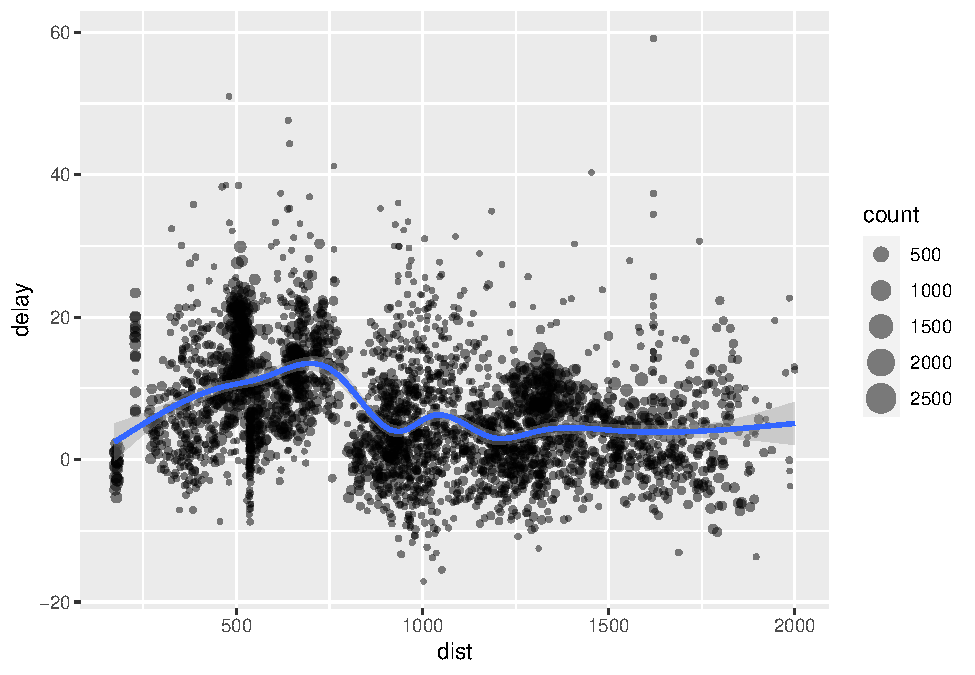
\includegraphics{DS-book-lab_files/figure-latex/unnamed-chunk-35-1.pdf}

\begin{enumerate}
\def\labelenumi{\arabic{enumi}.}
\setcounter{enumi}{7}
\tightlist
\item
  Знаходимо кількість літаків і кількість вильотів в усі можливі пункти призначення.
\end{enumerate}

\begin{Shaded}
\begin{Highlighting}[]
\NormalTok{destinations }\OtherTok{\textless{}{-}} \FunctionTok{group\_by}\NormalTok{(flights, dest)}
\FunctionTok{summarise}\NormalTok{(destinations,}
  \AttributeTok{planes =} \FunctionTok{n\_distinct}\NormalTok{(tailnum),}
  \AttributeTok{flights =} \FunctionTok{n}\NormalTok{()}
\NormalTok{)}
\end{Highlighting}
\end{Shaded}

\begin{verbatim}
## # A tibble: 105 x 3
##    dest  planes flights
##    <chr>  <int>   <int>
##  1 ABQ      108     254
##  2 ACK       58     265
##  3 ALB      172     439
##  4 ANC        6       8
##  5 ATL     1180   17215
##  6 AUS      993    2439
##  7 AVL      159     275
##  8 BDL      186     443
##  9 BGR       46     375
## 10 BHM       45     297
## # ... with 95 more rows
\end{verbatim}

\hypertarget{ux456ux43dux434ux438ux432ux456ux434ux443ux430ux43bux44cux43dux456-ux437ux430ux432ux434ux430ux43dux43dux44f-ux43dux430-ux43bux430ux431ux43eux440ux430ux442ux43eux440ux43dux443-ux440ux43eux431ux43eux442ux443-1}{%
\subsection{Індивідуальні завдання на лабораторну роботу}\label{ux456ux43dux434ux438ux432ux456ux434ux443ux430ux43bux44cux43dux456-ux437ux430ux432ux434ux430ux43dux43dux44f-ux43dux430-ux43bux430ux431ux43eux440ux430ux442ux43eux440ux43dux443-ux440ux43eux431ux43eux442ux443-1}}

Видає викладач.

\hypertarget{methods}{%
\chapter{Methods}\label{methods}}

We describe our methods in this chapter.

Math can be added in body using usual syntax like this

\hypertarget{math-example}{%
\section{math example}\label{math-example}}

\(p\) is unknown but expected to be around 1/3. Standard error will be approximated

\[
SE = \sqrt(\frac{p(1-p)}{n}) \approx \sqrt{\frac{1/3 (1 - 1/3)} {300}} = 0.027
\]

You can also use math in footnotes like this\footnote{where we mention \(p = \frac{a}{b}\)}.

We will approximate standard error to 0.027\footnote{\(p\) is unknown but expected to be around 1/3. Standard error will be approximated

  \[
  SE = \sqrt(\frac{p(1-p)}{n}) \approx \sqrt{\frac{1/3 (1 - 1/3)} {300}} = 0.027
  \]}

\hypertarget{applications}{%
\chapter{Applications}\label{applications}}

Some \emph{significant} applications are demonstrated in this chapter.

\hypertarget{example-one}{%
\section{Example one}\label{example-one}}

\hypertarget{example-two}{%
\section{Example two}\label{example-two}}

\hypertarget{final-words}{%
\chapter{Final Words}\label{final-words}}

We have finished a nice book.

  \bibliography{book.bib,packages.bib}

\end{document}
